\subsection{Contribution}

To ensure full transparency, the individual contributions of each team member are detailed below:

\begin{itemize}
    \item \textbf{Jan Sternberg:}
    \begin{itemize}
        \item \textbf{System Architecture \& Model Design:}
        \begin{itemize}
            \item Designed and implemented the core \texttt{AnimalClassifier} architecture based on an EfficientNetV2-S backbone initialized completely from scratch (\texttt{weights=None}), integrating a modified classification head with a regularized dropout probability \cite{tan2021efficientnetv2}.
            \item Developed a secondary \texttt{CompareClassifier} utilizing a pretrained ResNet18 model to serve as a baseline for performance comparisons \cite{kornblith2019transfer}.
        \end{itemize}
        \item \textbf{Object Detection \& Spatial Preprocessing:}
        \begin{itemize}
            \item Integrated the YOLOv6 object detection framework via PyTorch Hub to automatically localize and crop the largest target animal (distinguishing between cat species ID 15 and dog species ID 16) to a standardized resolution \cite{li2022yolov6}.
            \item Implemented automated weight-download routines and robust checkpoint-loading mechanisms featuring security patches for modern PyTorch serialization standards (\texttt{weights\_only=False}) \cite{paszke2019pytorch}.
            \item Formulated a data-shuffling and structuring script to automatically organize raw image directories into sequential, ID-based file structures paired with a unified CSV labeling system.
        \end{itemize}
        \item \textbf{Dataset Engineering \& Multi-Source Integration:}
        \begin{itemize}
            \item Developed and executed automated data collection and integration pipelines across multiple benchmark repositories, including the Oxford-IIIT Pet Dataset \cite{parkhi2012catsdogs}, Stanford Dogs Dataset \cite{khosla2011novel}, Kaggle cat breeds \cite{deng2009imagenet}, and The Cat API \cite{cat_api}.
            \item Implemented robust checkpoint-aware file counters and duplicate-prevention mechanisms (\texttt{get\_next\_counter}) to safely merge local classes and external image archives into a unified, clean dataset structure.
        \end{itemize}
        \item \textbf{Advanced Training Pipelines, SLURM Job Management \& Execution:}
        \begin{itemize}
            \item Engineered a high-performance training script featuring offline spatial caching, automatic mixed precision (AMP) via PyTorch \texttt{grad\_scaler}, AdamW optimization, and Cosine Annealing learning rate schedules \cite{paszke2019pytorch}.
            \item Configured, scheduled, and managed comprehensive batch training jobs on high-performance computing clusters using \textbf{SLURM}, setting up persistent error/output logging (\texttt{.log} files) and monitoring active runs.
            \item Developed custom data augmentation routines—including horizontal mirroring, Gaussian blurring, and a localized multi-scale patch regularization method (\texttt{CropMix})—to improve model generalization \cite{yun2019cutmix}.
            \item Implemented automated handling of class imbalances via dynamic class-weight calculations in CrossEntropyLoss, as well as alternative multi-GPU scaling scripts leveraging \texttt{nn.DataParallel}, learning rate warmups, and weighted random sampling \cite{paszke2019pytorch}.
        \end{itemize}
        \item \textbf{Evaluation, Explainable AI (Heatmaps) \& Performance Visualization:}
        \begin{itemize}
            \item Built an automated evaluation utility to parse multiple \texttt{.pth} checkpoint files, inspect tensor structures, and extract detailed validation and per-class accuracy metrics.
            \item Implemented an advanced Explainable AI (XAI) tool using \textbf{Grad-CAM} to dynamically compute target convolutional feature layers, extract top predicted class indices, and generate thermal \textbf{heatmaps} overlaid onto test images with automatic directory creation and sequential naming conventions (\texttt{CAM\_Heat\_Map}) \cite{selvaraju2017grad}.
            \item Created an automated logging, regex-parsing, and graphing pipeline to visualize multi-epoch \textbf{loss and accuracy curves} (e.g., tracking training vs. validation performance, highlighting optimal checkpoints and maximum validation accuracies) \cite{prechelt1998early}.
        \end{itemize}
        \item \textbf{Documentation \& Project Structuring:}
        \begin{itemize}
            \item Structured, drafted, and authored the comprehensive final project report and documentation, outlining the end-to-end computer vision pipeline, experimental setups, hyperparameter configurations, quantitative evaluations, and visual interpretability insights.
        \end{itemize}
    \end{itemize}

    \item \textbf{Marc Koester:}
    \begin{itemize}
        \item \textbf{Project Organization \& Leadership:}
        \begin{itemize}
            \item Organized the project infrastructure, set up the Discord channel, and planned regular group meetings.
        \end{itemize}
        \item \textbf{Dataset Expansion \& Balancing:}
        \begin{itemize}
            \item Added 6,000 pictures to the dataset to complement cat and dog classes that were lacking sufficient training data.
            \item Coded the class-imbalance argument and implemented a command-line solution using \texttt{--} to handle class imbalances for breeds with skewed image distributions.
        \end{itemize}
        \item \textbf{Data Testing \& Exploration:}
        \begin{itemize}
            \item Tested both old and new dataset versions on Kaggle and explored AI-generated image options.
        \end{itemize}
        \item \textbf{Presentation \& Formatting:}
        \begin{itemize}
            \item Led the presentation creation, structured the slides, gave everyone a rough script, and implemented a coherent design across all presentation slides.
        \end{itemize}
    \end{itemize}


    \begin{itemize}
        \item \textbf{Ivan Kazakov:}
        \begin{itemize}
            \item \textbf{Dataset Acquisition \& Curation:}
            \begin{itemize}
                \item Sourced core breed datasets after the initial API approach proved insufficient: the Kaggle cat-breed dataset ($\sim$1,000 images/class), the Tsinghua Dogs dataset, and a Dalmatian subset from an additional Kaggle dog dataset.
                \item Assembled and published the merged $\sim$26k-image / 20-class training dataset on Kaggle.
            \end{itemize}
            \item \textbf{Training Pipeline \& Scaling:}
            \begin{itemize}
                \item Collaborated on the EfficientNetV2-S training pipeline development.
                \item Scaled training infrastructure from a single P100 to 2x T4 GPUs using DataParallel; identified, diagnosed, and mitigated CPU-side image decoding bottlenecks.
            \end{itemize}
            \item \textbf{Model Development \& Experiments:}
            \begin{itemize}
                \item Trained the combined 20-class model achieving 84.9\% test accuracy (macro F1 0.829) with pretrained initialization, as well as the required from-scratch baseline (80 epochs, 78.1\% / 0.752), providing the comparative results for the report.
                \item Co-implemented the species-split architecture (separate cat and dog models via class presets) and analyzed the dogs-vs-cats transfer asymmetry alongside its ImageNet class-composition background.
                \item Evaluated a community cat-breed checkpoint as an alternative initialization strategy and integrated a robust checkpoint-format loader.
            \end{itemize}
            \item \textbf{System Integration \& Inference:}
            \begin{itemize}
                \item Supported the end-to-end evaluation and error analysis framework that contributed to securing the group's first-place challenge submission (73.28\%).
            \end{itemize}
            \item \textbf{Report \& Presentation:}
            \begin{itemize}
                \item Delivered presentation segments covering data acquisition, training setups, and the pretrained-vs-scratch comparison; produced corresponding training-curve and performance comparison figures.
                \item Cowrote the System Architecture, Classification Model, and Integration Findings part of the final paper in the experiments and Related Work section
                \item Published both pipeline editions (combined and species-split) as fully documented repositories and notebooks.
            \end{itemize}
        \end{itemize}
    \end{itemize}

    \item \textbf{Huang Ziyang:}
    \begin{itemize}
        \item Created and initialized the collaborative repository.
        \item Proofread the final paper.
        \item Compared the AdamW vs. the Ranger optimizer for the presentation.
        \item Created first Draft of the README.md
    \end{itemize}
\end{itemize}
%

\subsection{Code and Environment Reproducibility}
\label{sec:code_reproducibility}

The complete source code, trained model checkpoints, and inference scripts are hosted in our repository:
\begin{center}
    \href{https://github.com/NordlichtS/CVDL26-drop-table-catdogs}{CVDL26-drop-table-catdogs}
\end{center}
Please refer to the repository README file for environment setup instructions and data preparation steps.


\subsection{Detailed Training History Curves}
\label{sec:appendix_curves}

This appendix presents the full training and validation loss alongside accuracy progression curves across all seven experimental configurations for both Cat and Dog datasets.

\begin{figure*}[htbp]
    \centering
    % Task 1: Baseline (Standard)
    \begin{subfigure}[b]{0.48\textwidth}
        \centering
        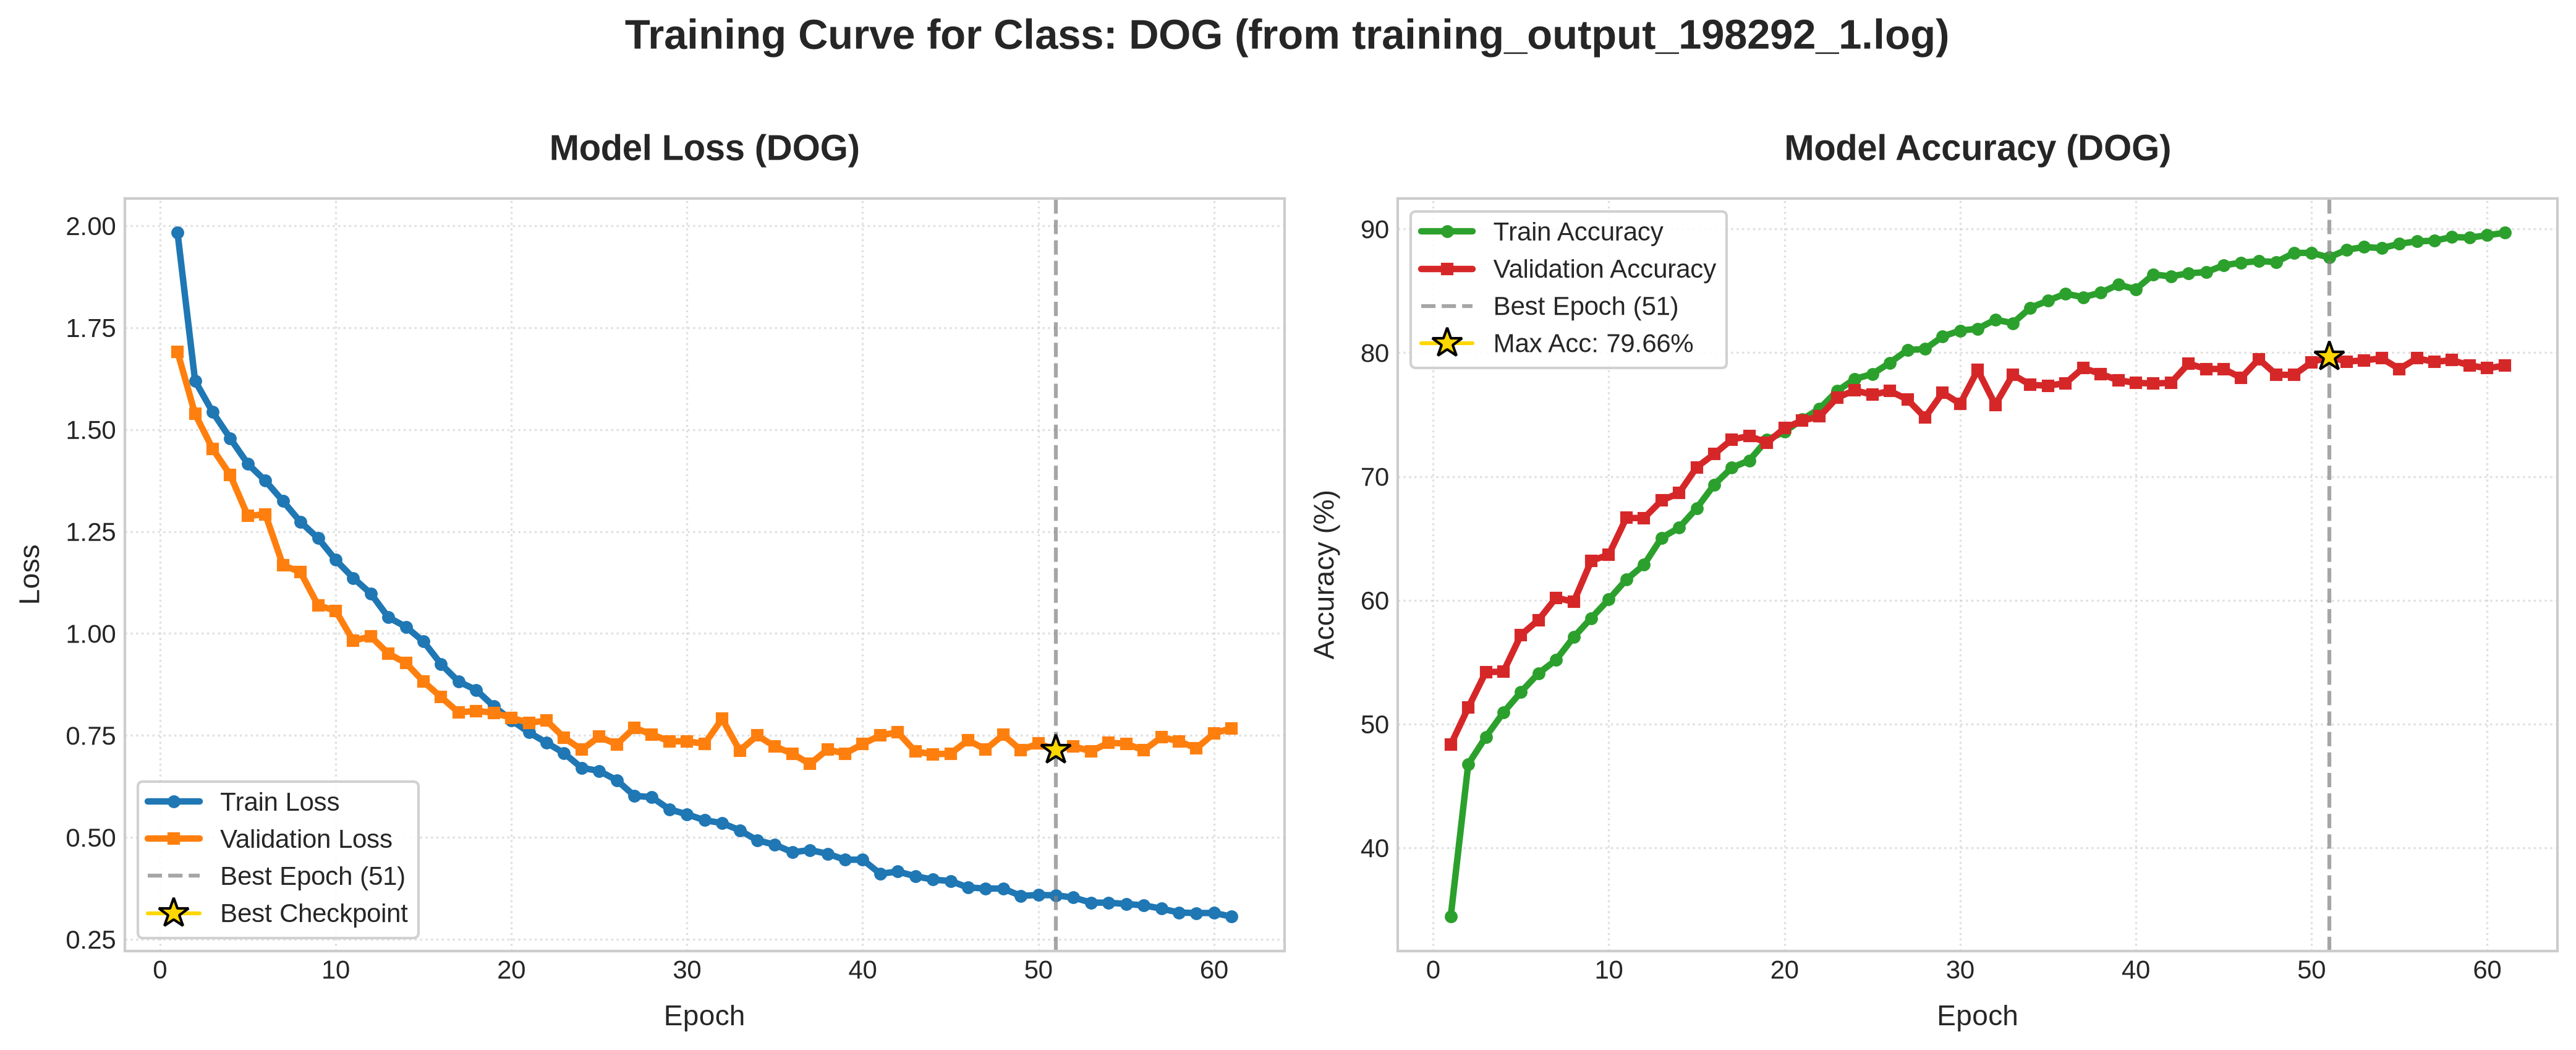
\includegraphics[width=\textwidth]{../Epoch/loss_Graphs/training_output_198292_1_dog.png}
        \caption{Task 1: Dog Baseline ($\text{LR}=1\times 10^{-5}$, 100 Ep.)}
    \end{subfigure}
    \hfill
    \begin{subfigure}[b]{0.48\textwidth}
        \centering
        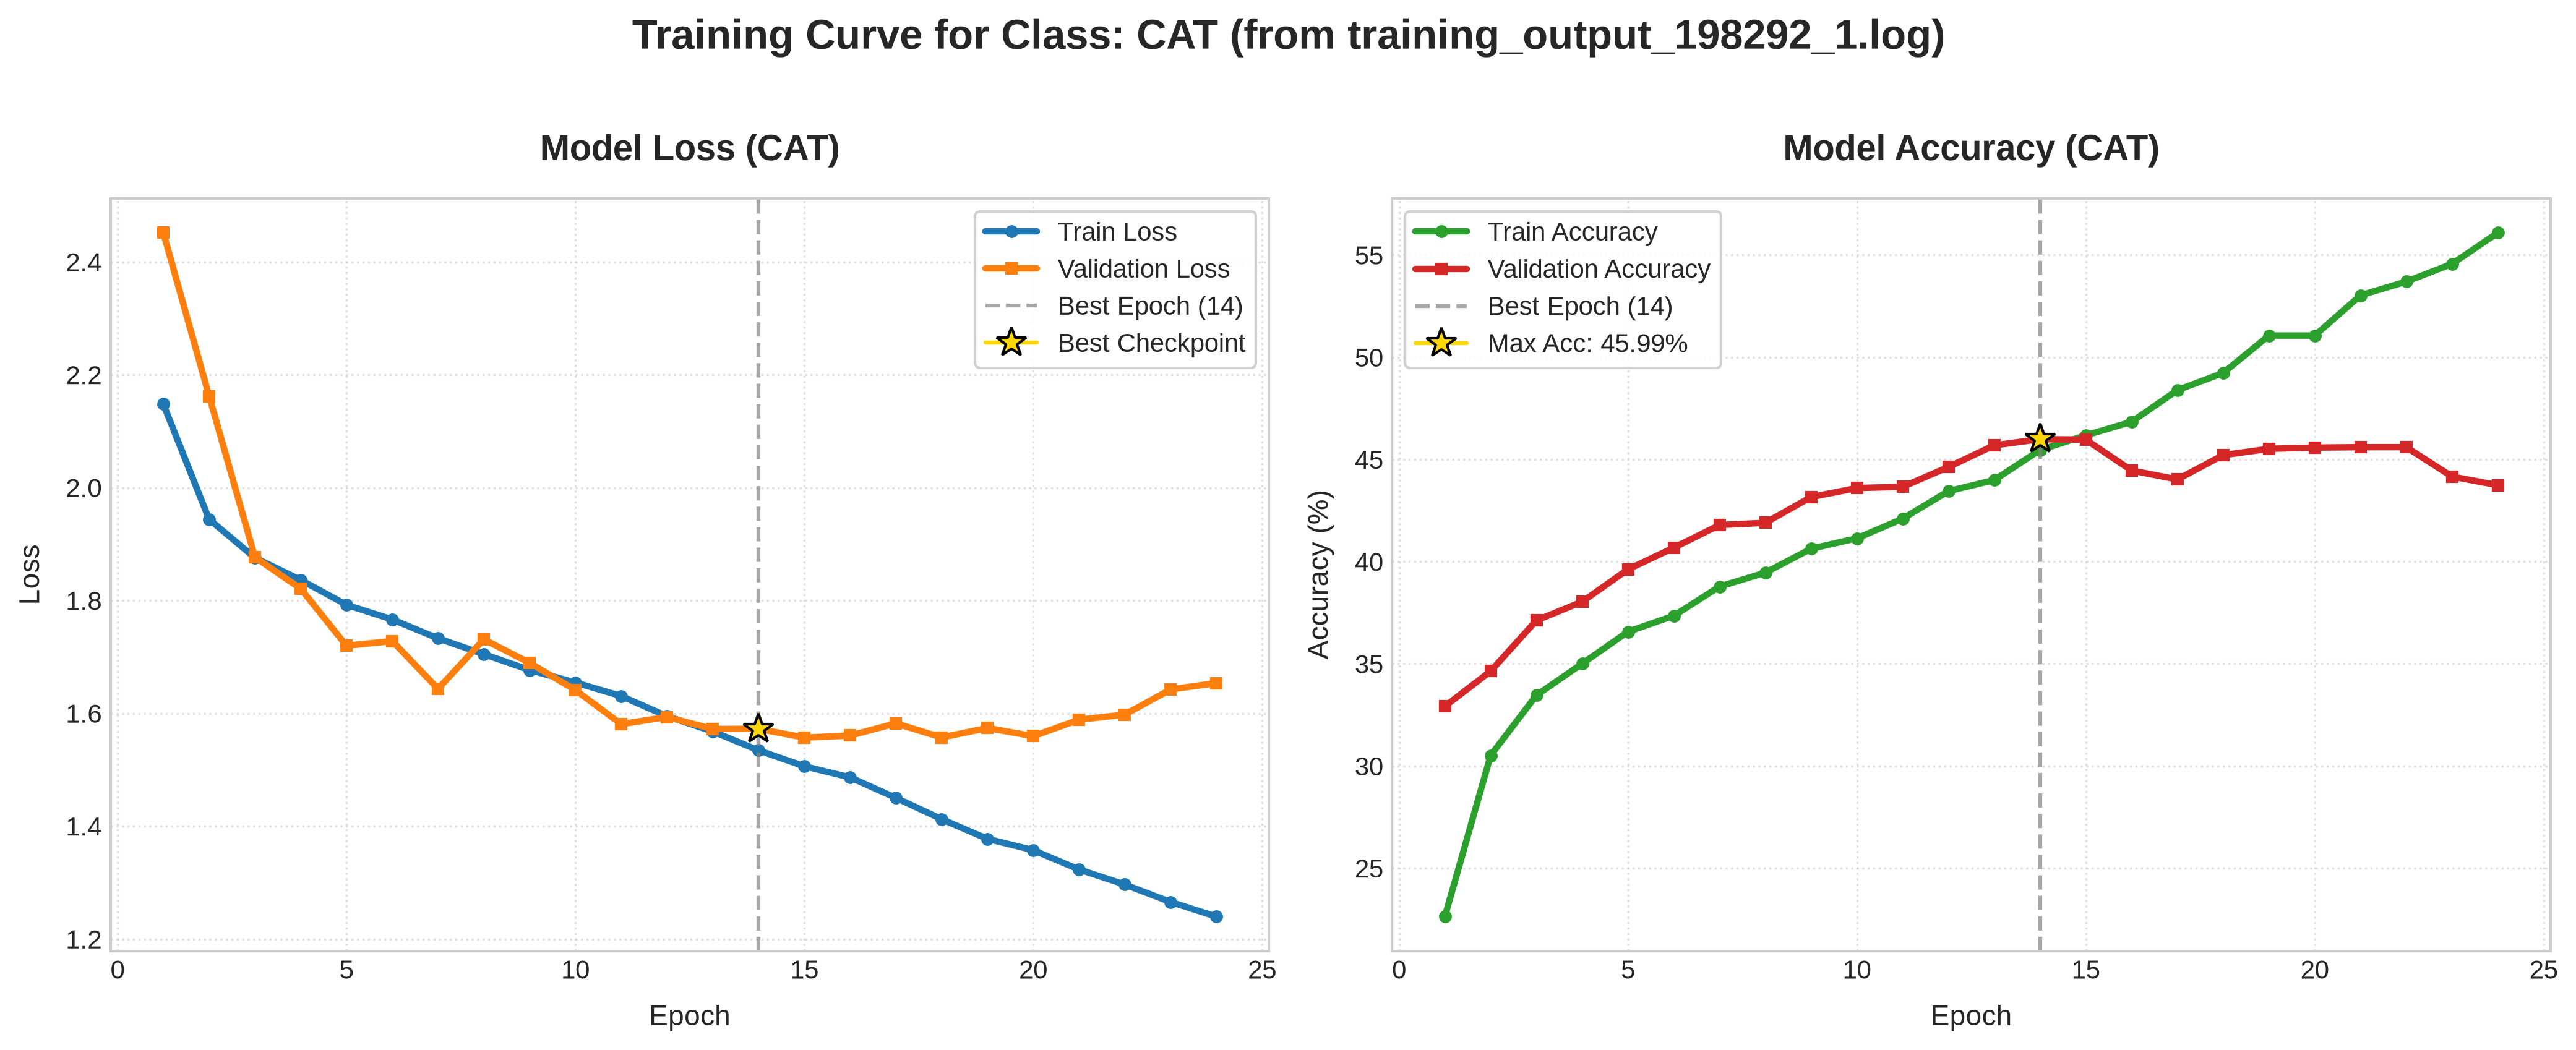
\includegraphics[width=\textwidth]{../Epoch/loss_Graphs/training_output_198292_1_cat.png}
        \caption{Task 1: Cat Baseline ($\text{LR}=1\times 10^{-5}$, 100 Ep.)}
    \end{subfigure}
    
    \vspace{0.3cm}
    
    % Task 2: Balanced Weights
    \begin{subfigure}[b]{0.48\textwidth}
        \centering
        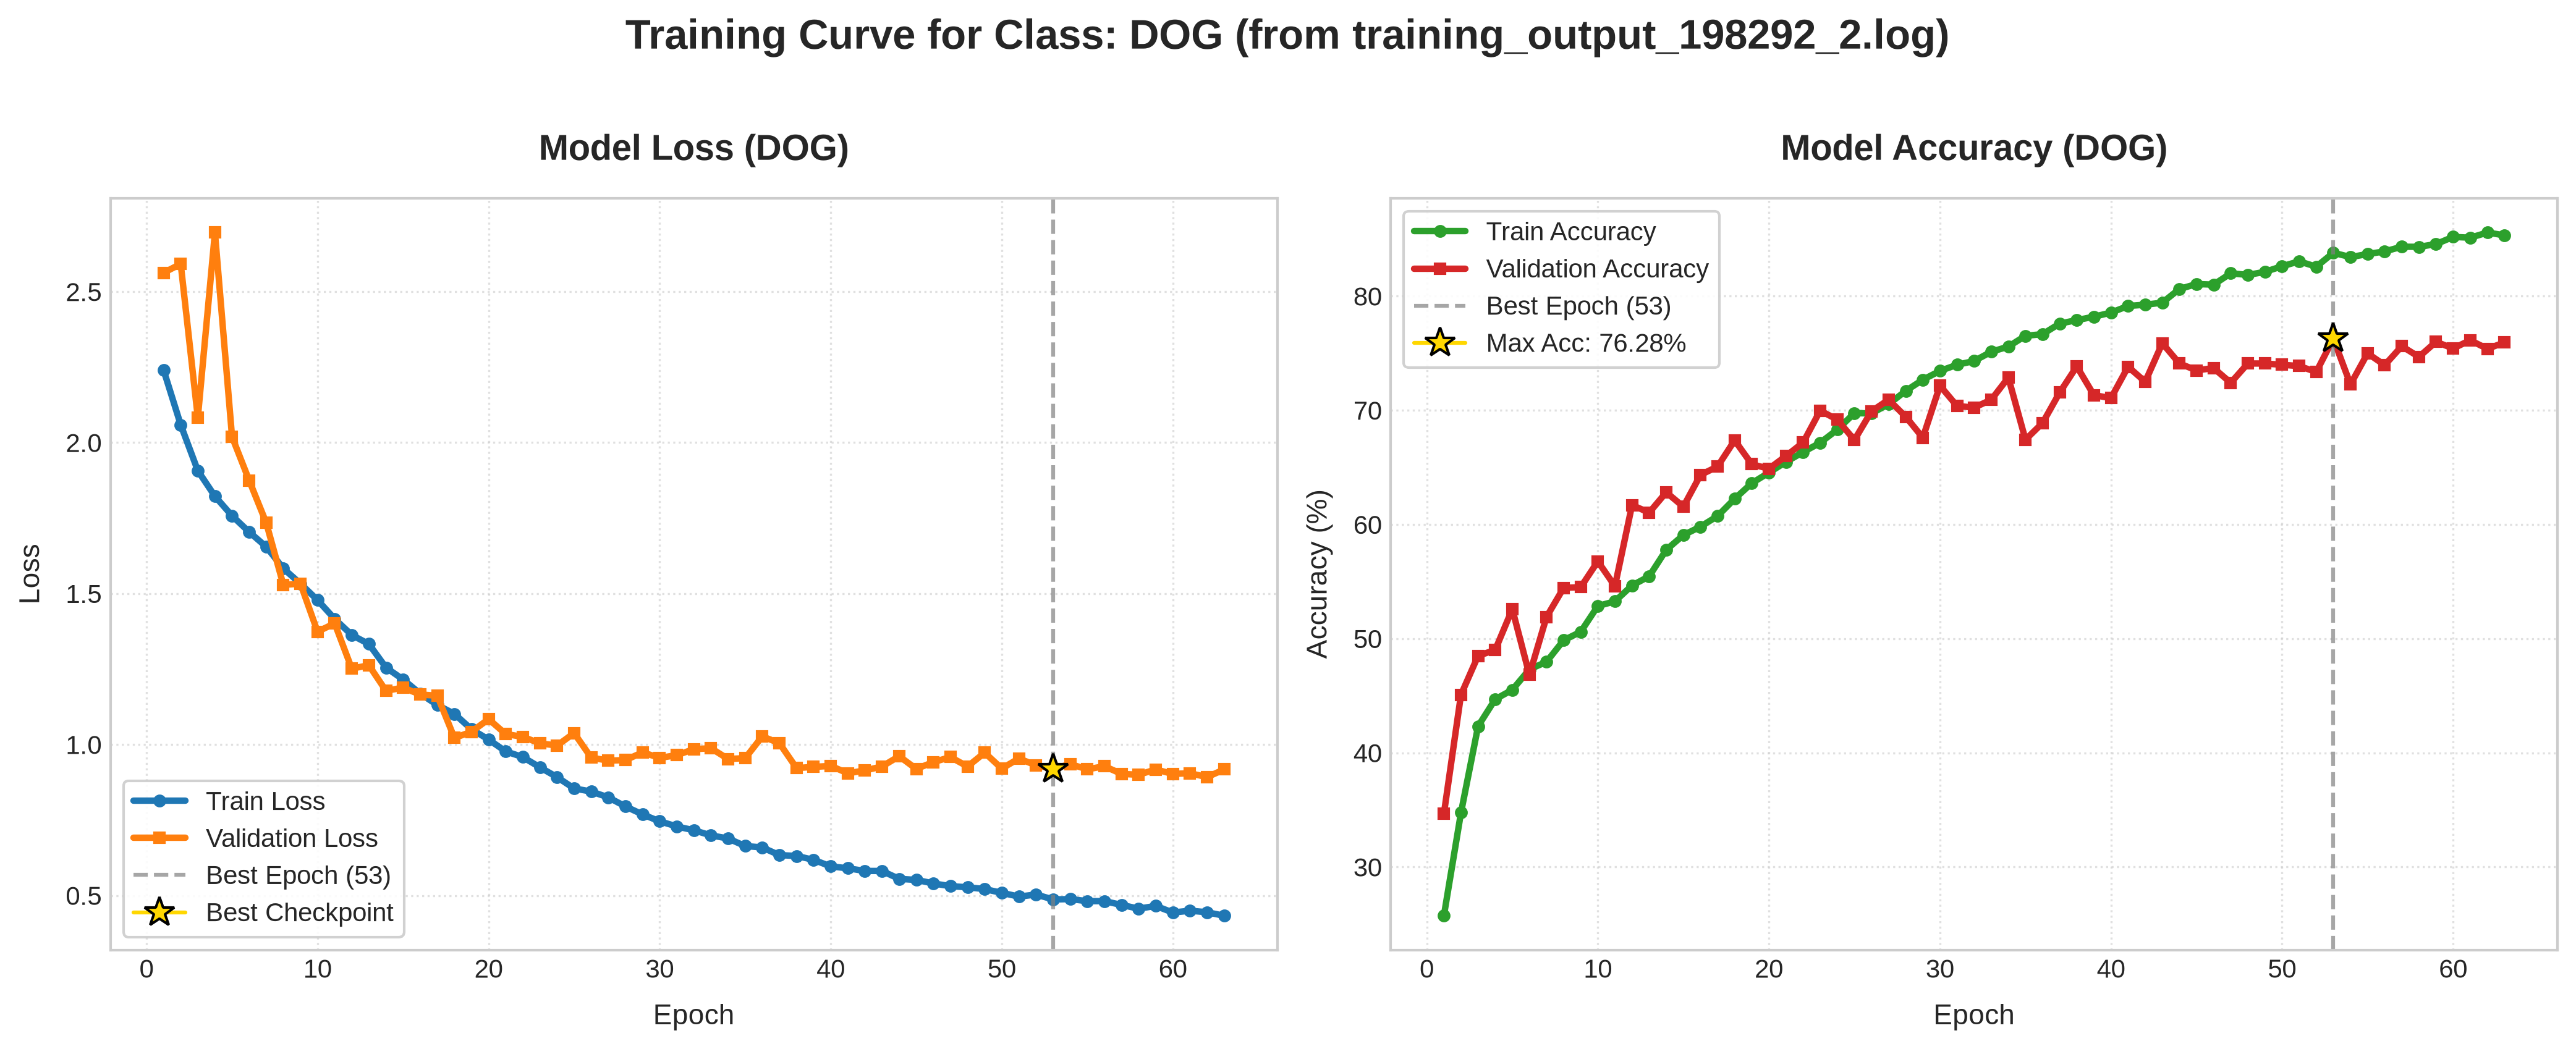
\includegraphics[width=\textwidth]{../Epoch/loss_Graphs/training_output_198292_2_dog.png}
        \caption{Task 2: Dog Balanced Weights ($\text{LR}=1\times 10^{-5}$, 100 Ep.)}
    \end{subfigure}
    \hfill
    \begin{subfigure}[b]{0.48\textwidth}
        \centering
        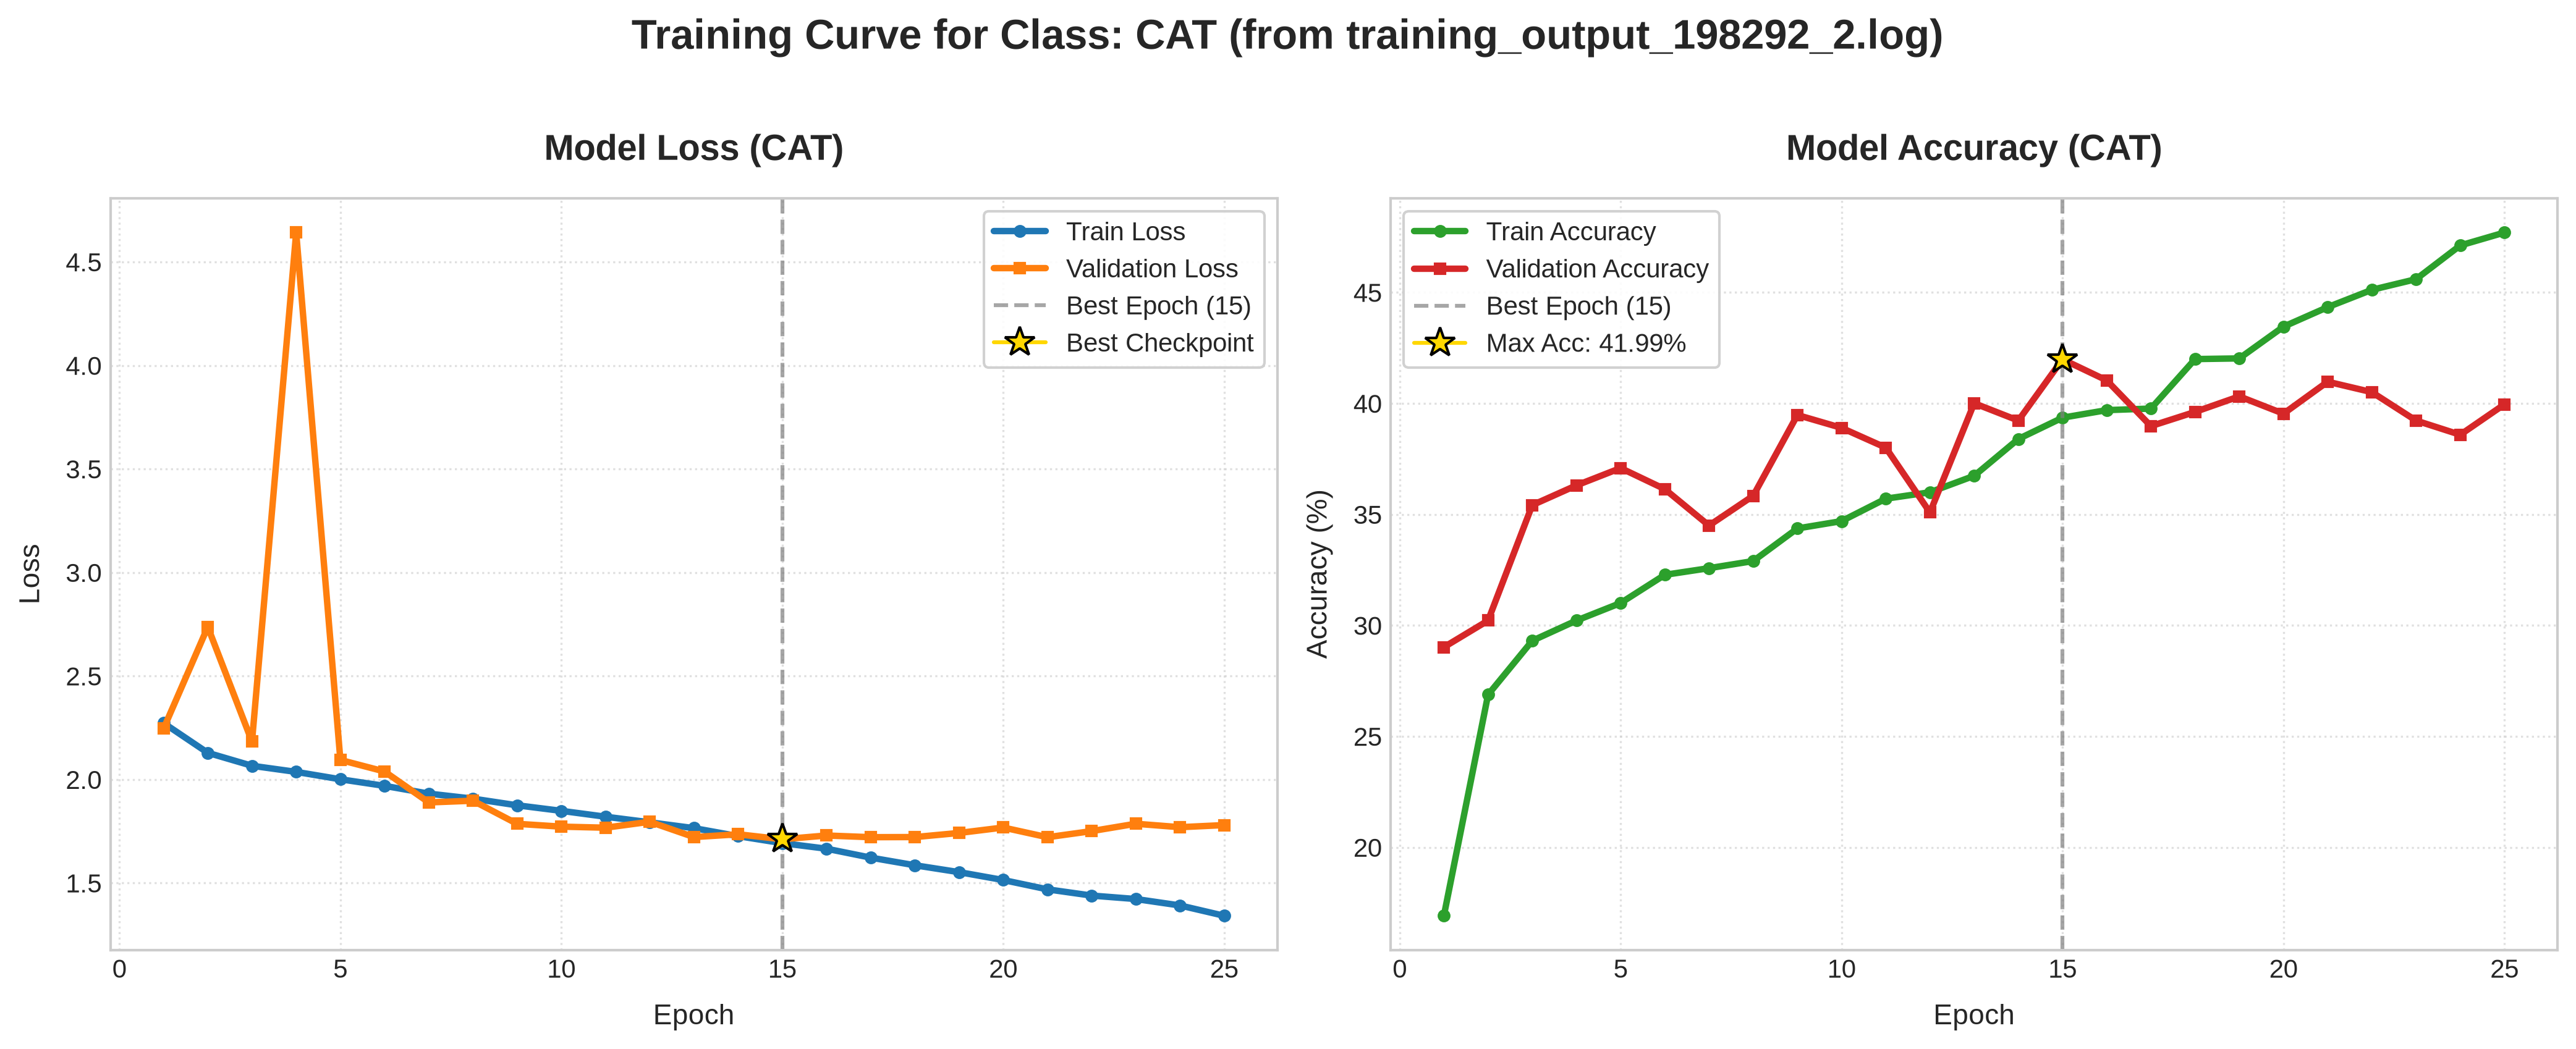
\includegraphics[width=\textwidth]{../Epoch/loss_Graphs/training_output_198292_2_cat.png}
        \caption{Task 2: Cat Balanced Weights ($\text{LR}=1\times 10^{-5}$, 100 Ep.)}
    \end{subfigure}

    \vspace{0.3cm}

    % Task 3: Blur
    \begin{subfigure}[b]{0.48\textwidth}
        \centering
        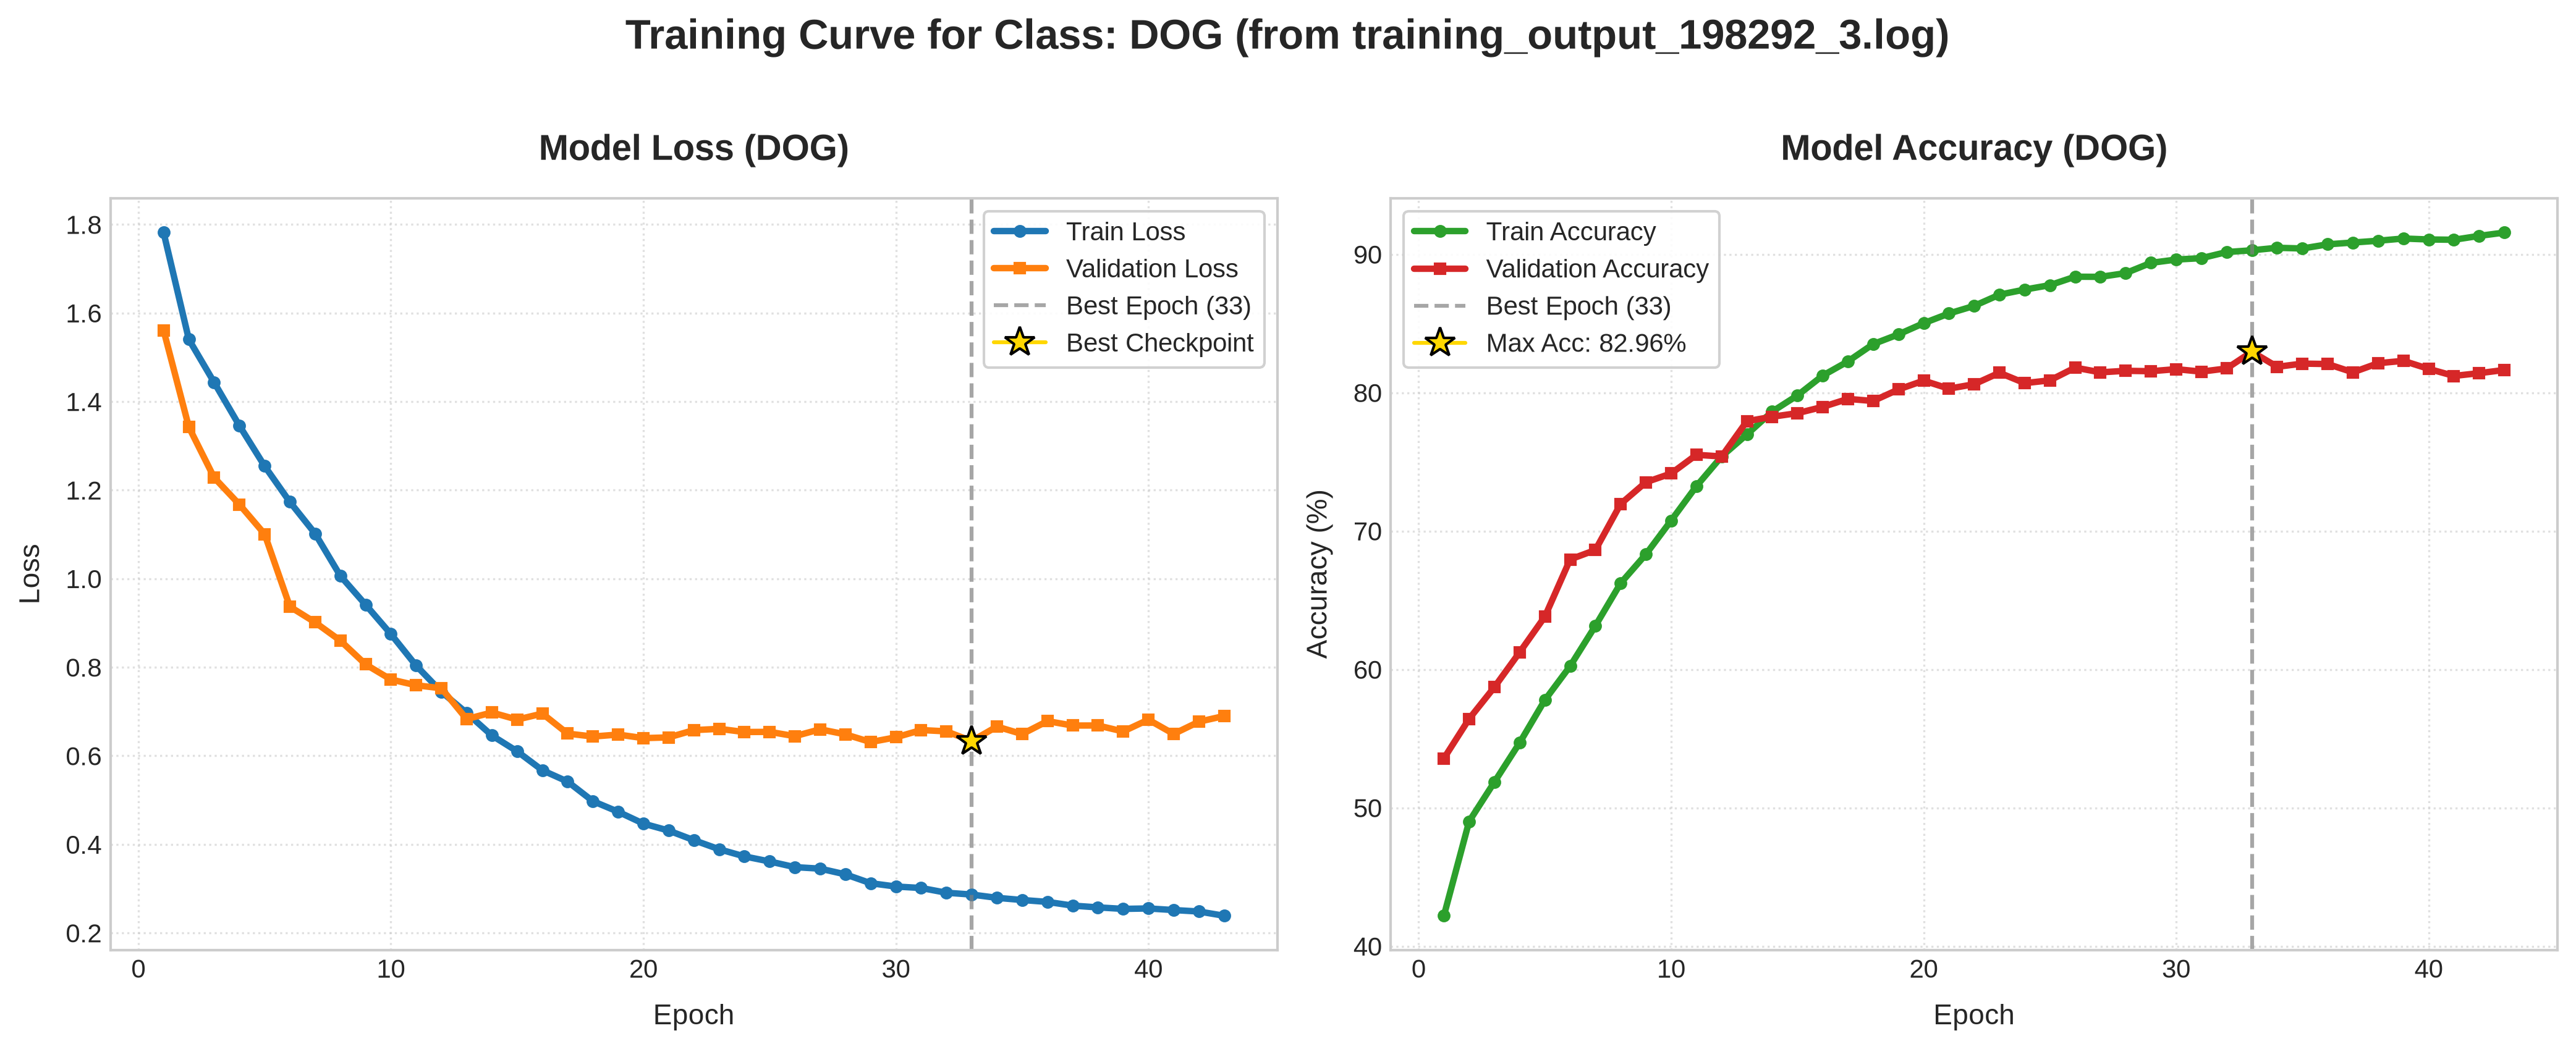
\includegraphics[width=\textwidth]{../Epoch/loss_Graphs/training_output_198292_3_dog.png}
        \caption{Task 3: Dog Blur ($\text{LR}=1\times 10^{-5}$, 100 Ep., $82.96\%$)}
    \end{subfigure}
    \hfill
    \begin{subfigure}[b]{0.48\textwidth}
        \centering
        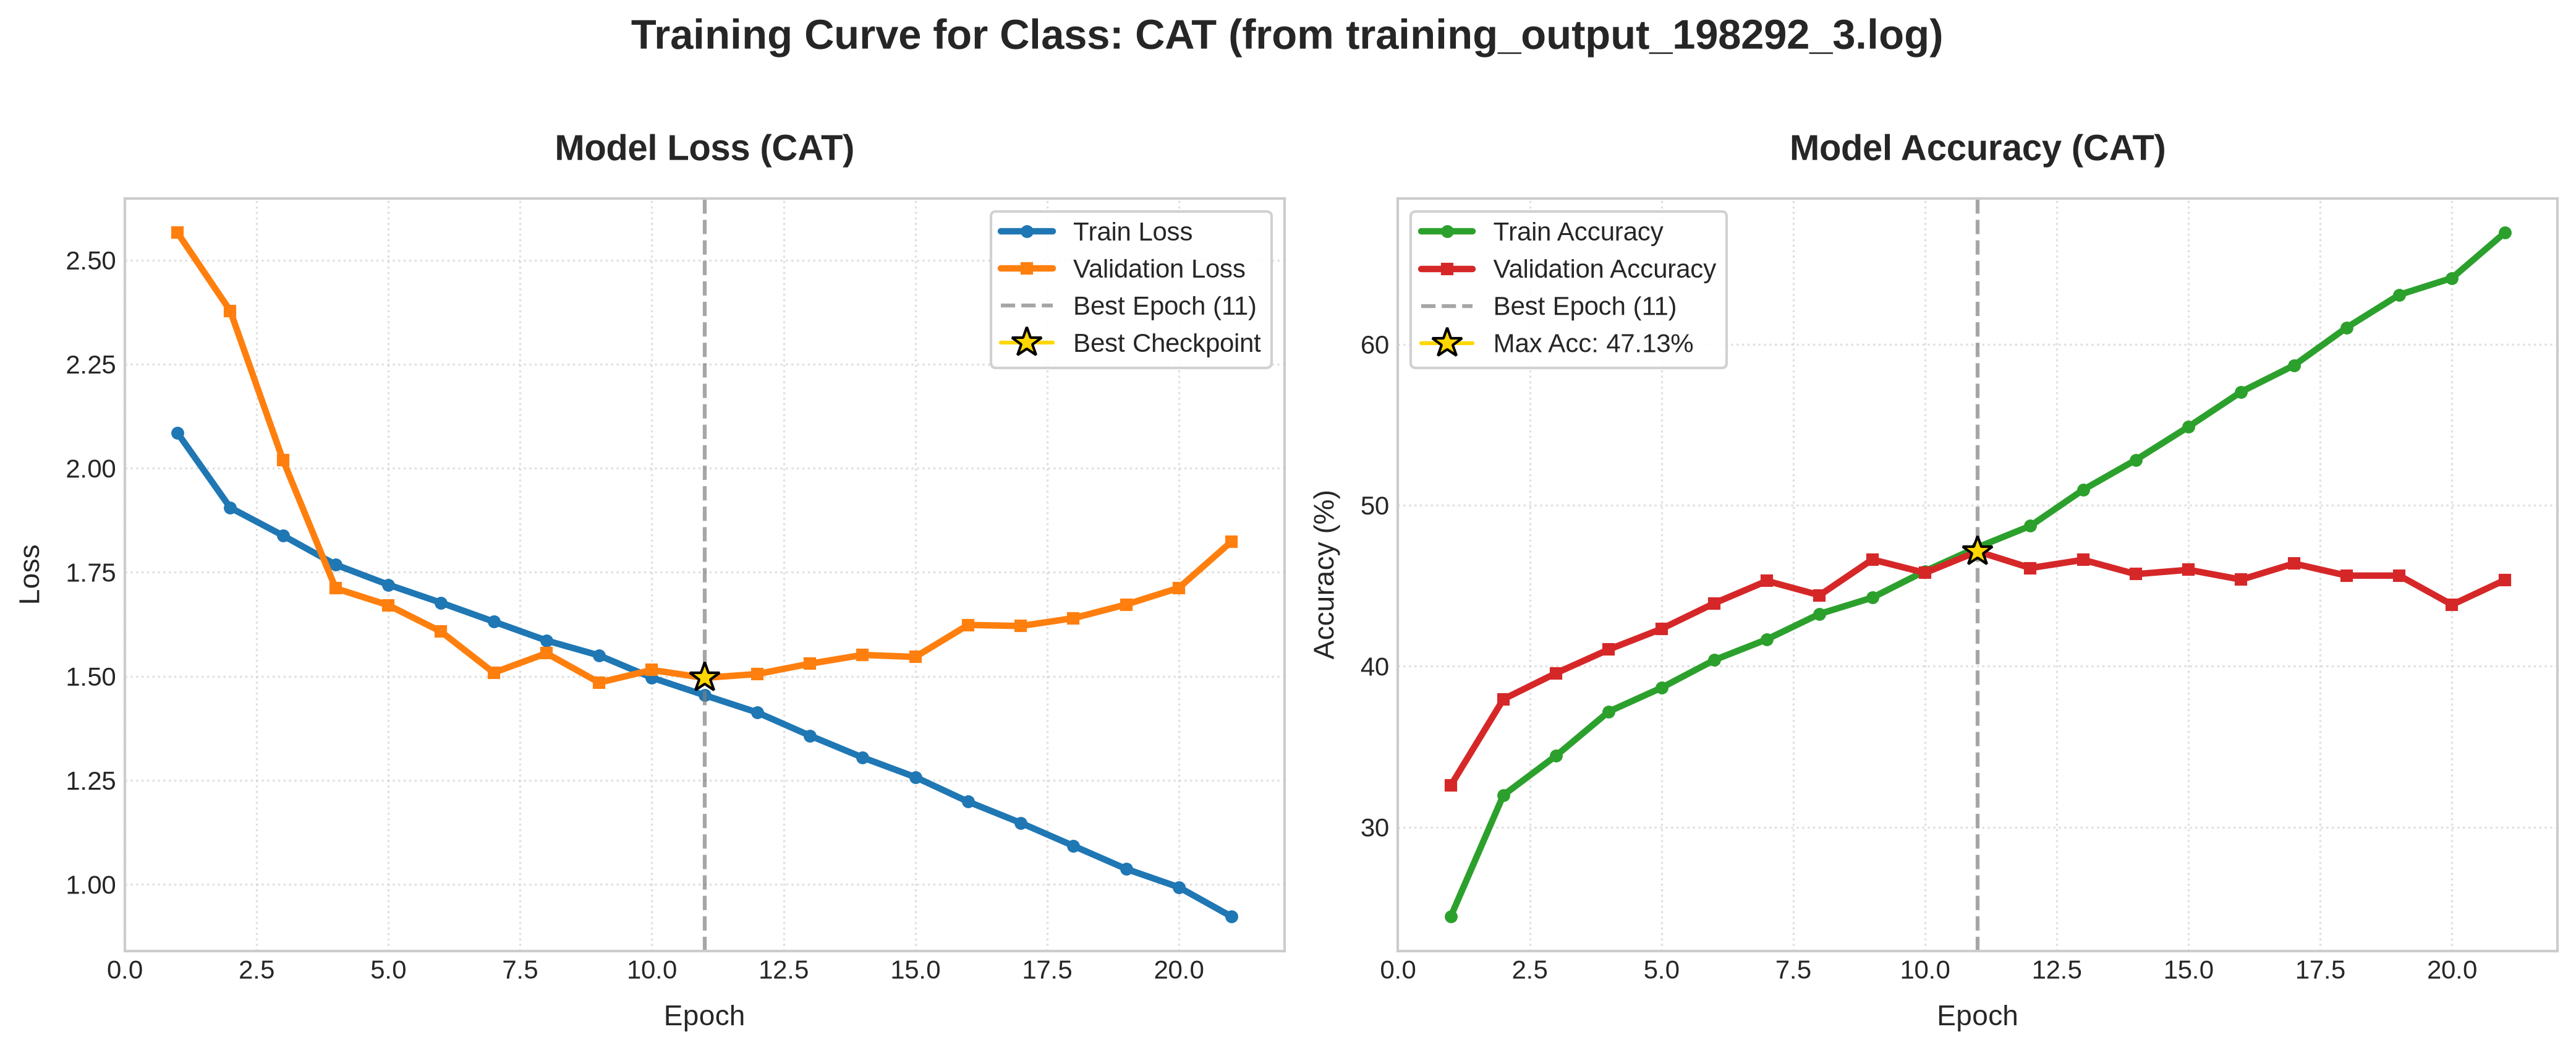
\includegraphics[width=\textwidth]{../Epoch/loss_Graphs/training_output_198292_3_cat.png}
        \caption{Task 3: Cat Blur ($\text{LR}=1\times 10^{-5}$, 100 Ep., $47.13\%$)}
    \end{subfigure}

    \vspace{0.3cm}

    % Task 4: Mirror
    \begin{subfigure}[b]{0.48\textwidth}
        \centering
        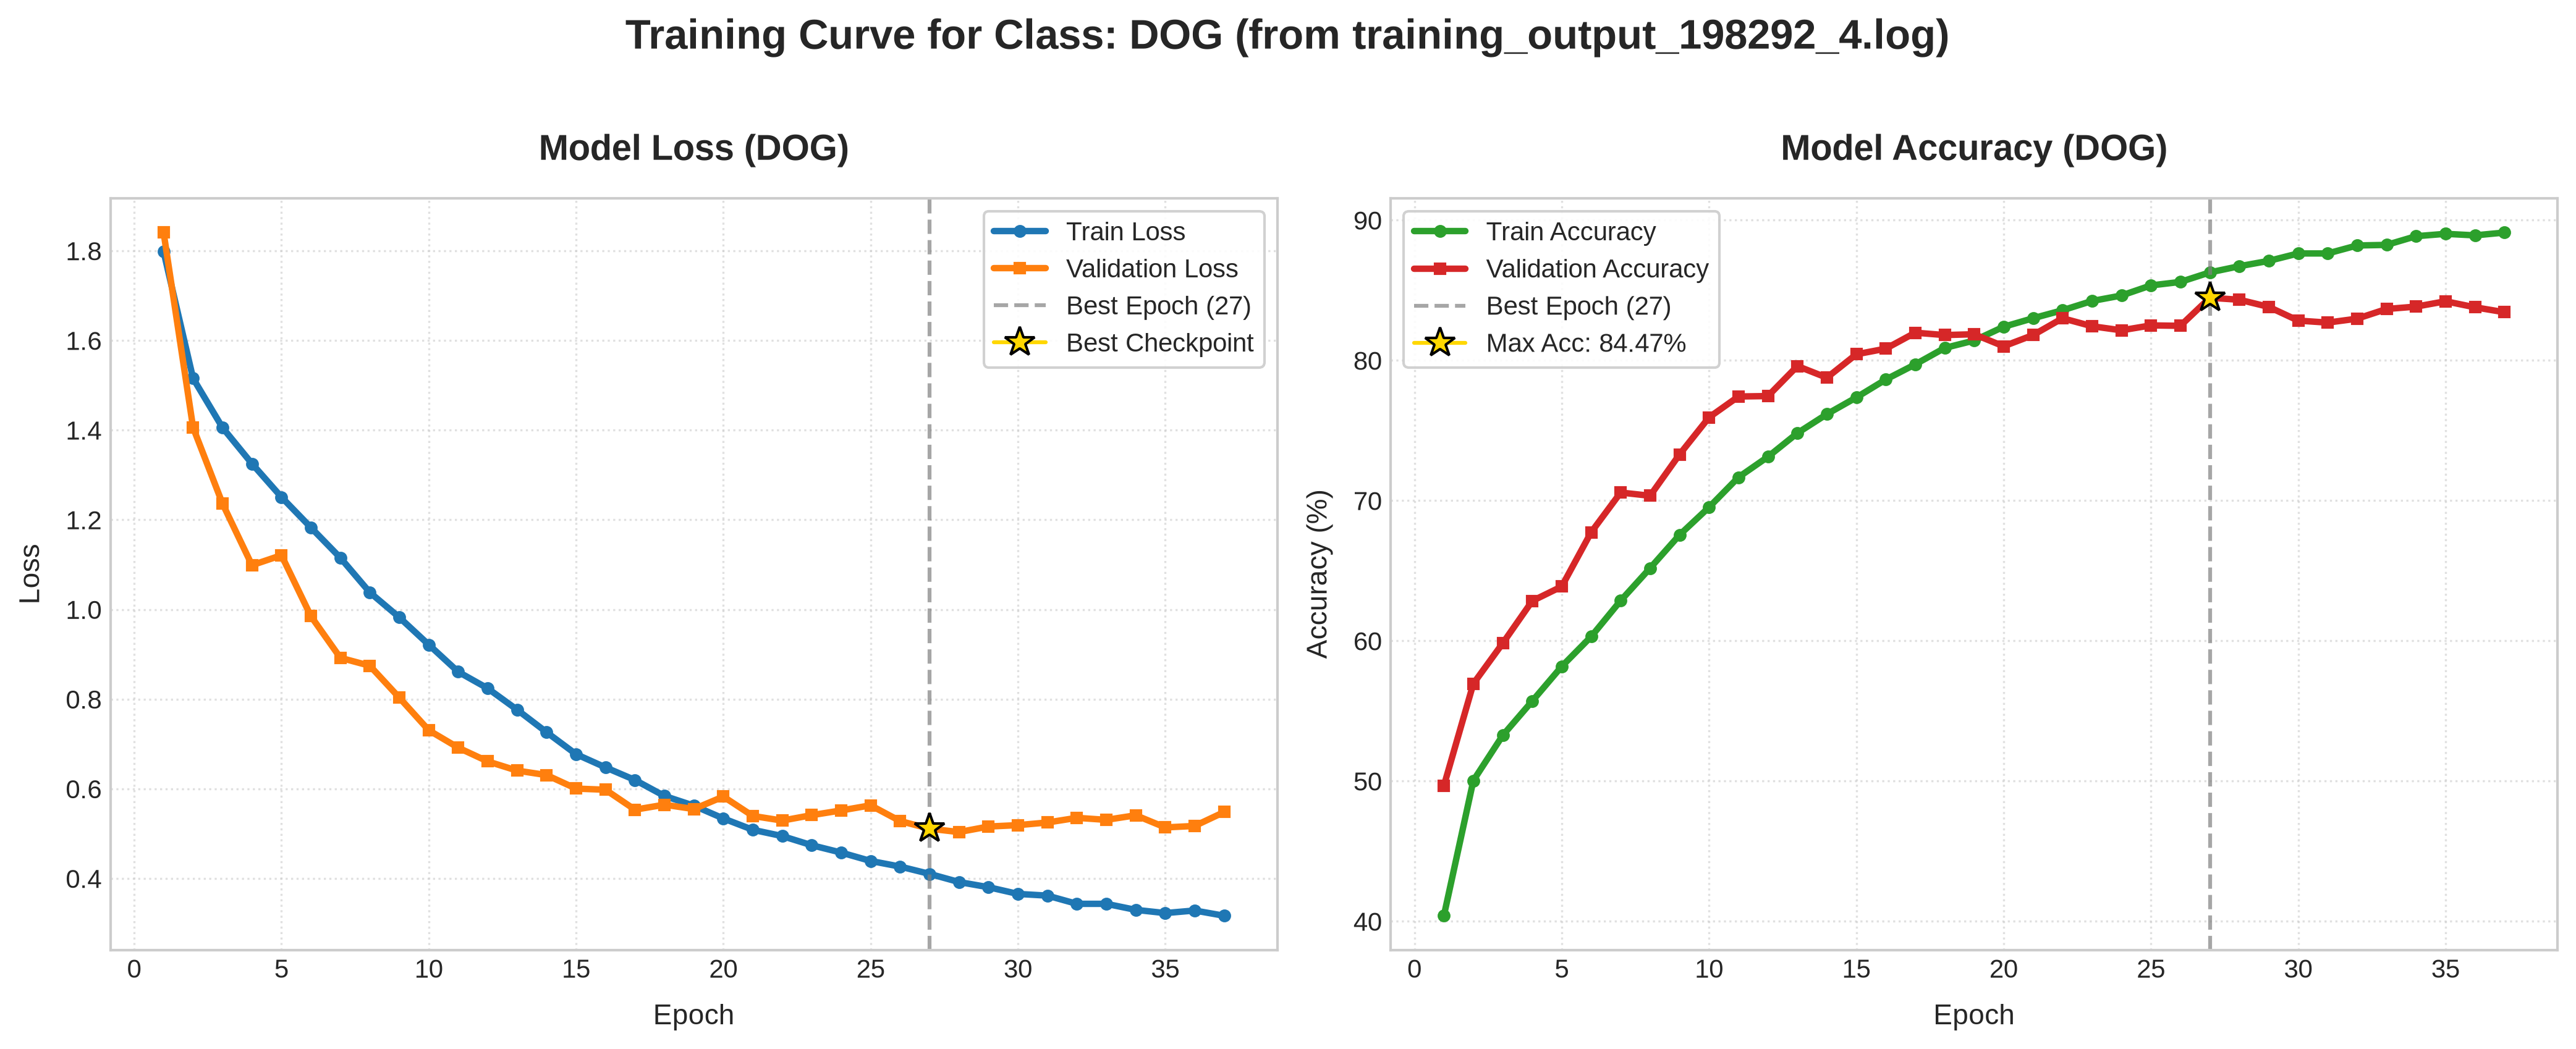
\includegraphics[width=\textwidth]{../Epoch/loss_Graphs/training_output_198292_4_dog.png}
        \caption{Task 4: Dog Mirror ($\text{LR}=1\times 10^{-5}$, 100 Ep.)}
    \end{subfigure}
    \hfill
    \begin{subfigure}[b]{0.48\textwidth}
        \centering
        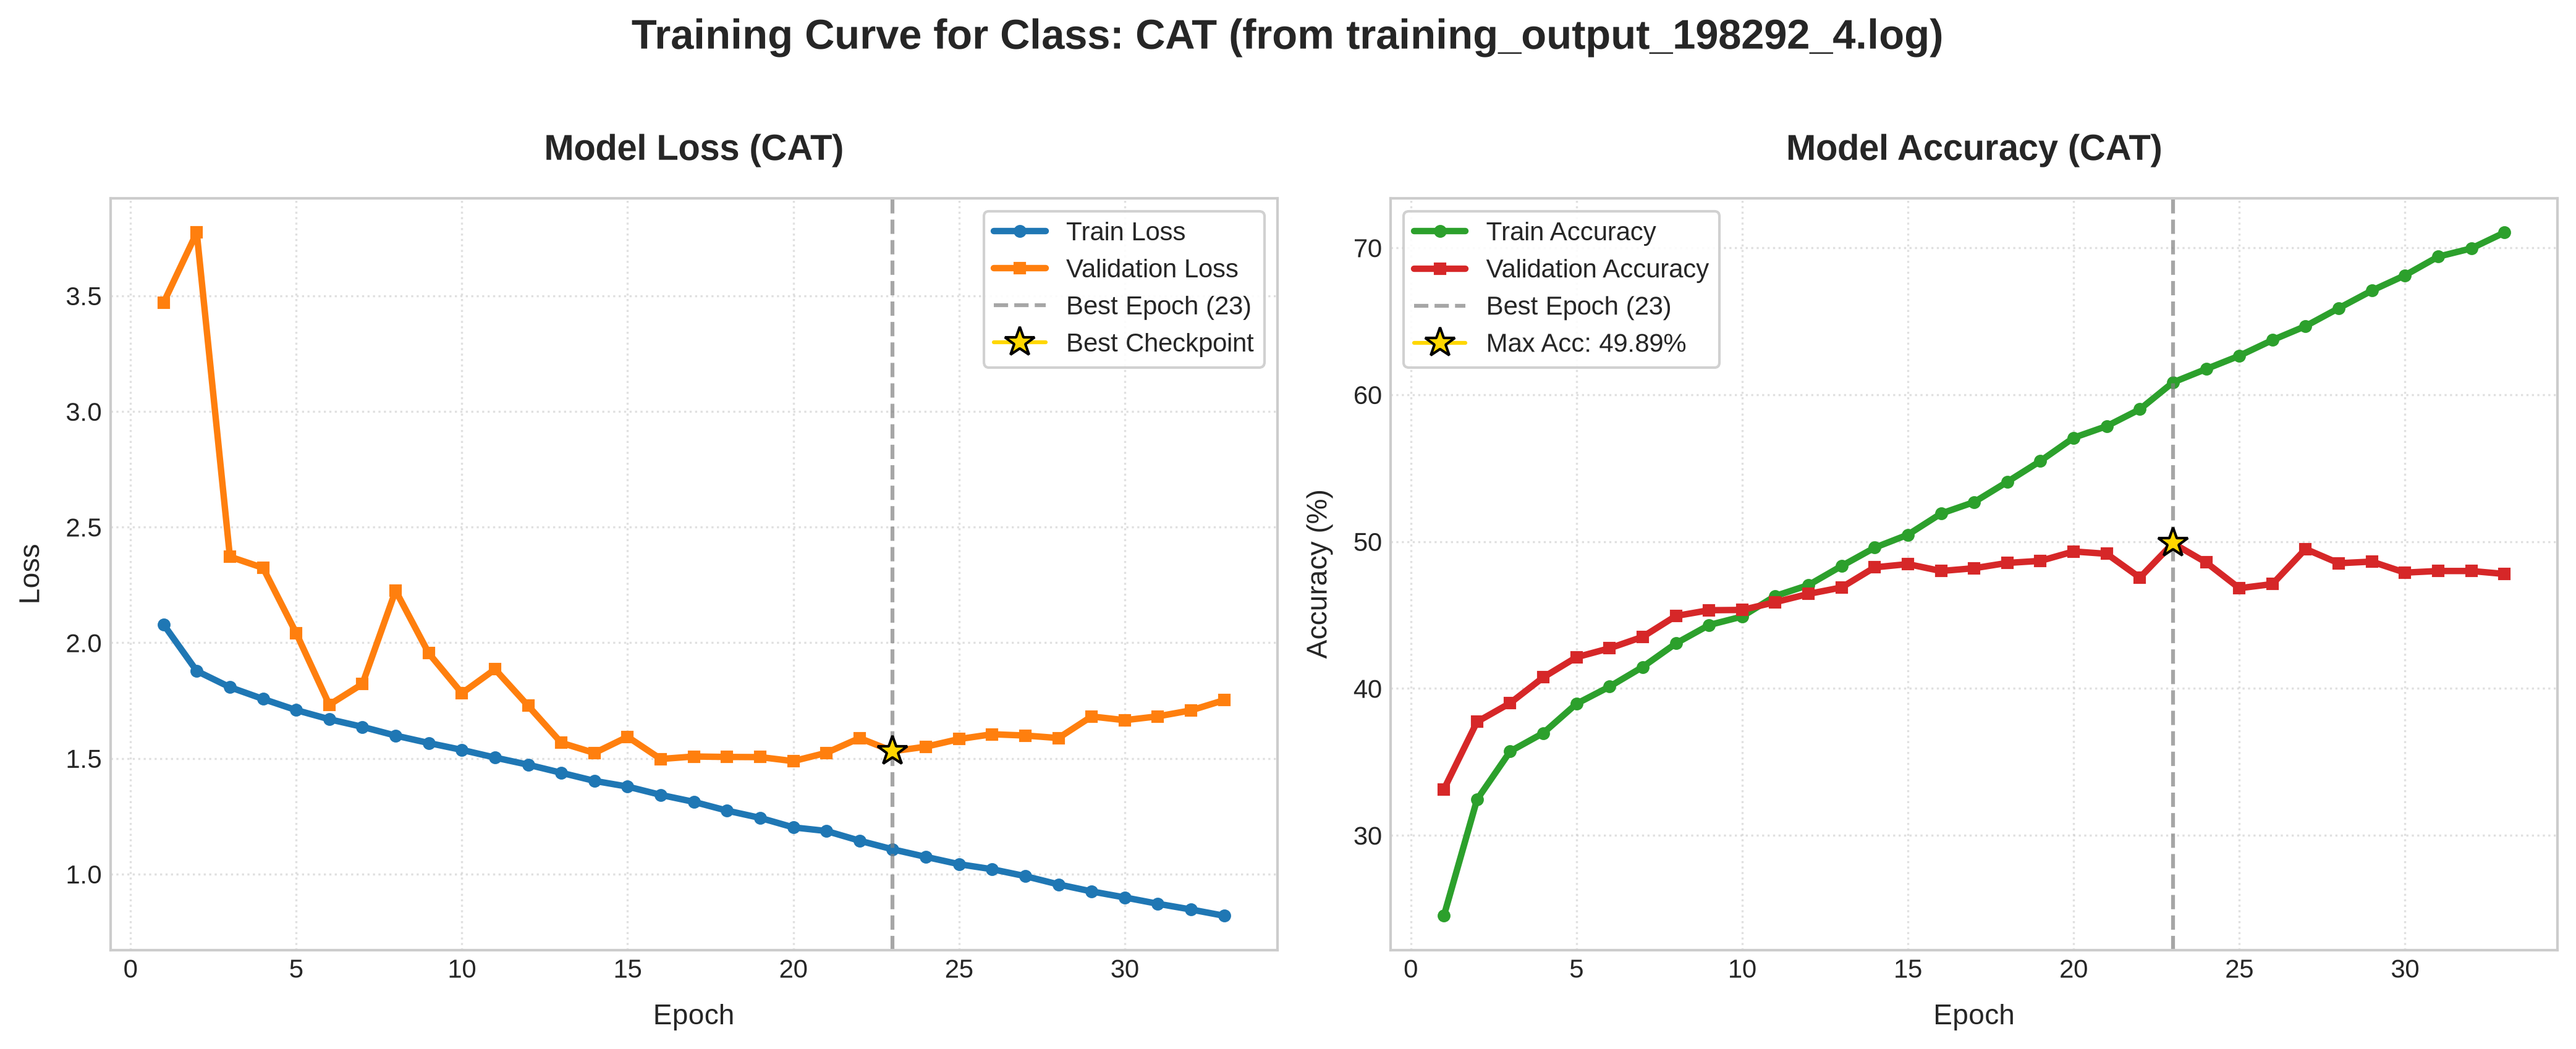
\includegraphics[width=\textwidth]{../Epoch/loss_Graphs/training_output_198292_4_cat.png}
        \caption{Task 4: Cat Mirror ($\text{LR}=1\times 10^{-5}$, 100 Ep., $49.89\%$)}
    \end{subfigure}

    \vspace{0.3cm}

    % Task 5: CropMix
    \begin{subfigure}[b]{0.48\textwidth}
        \centering
        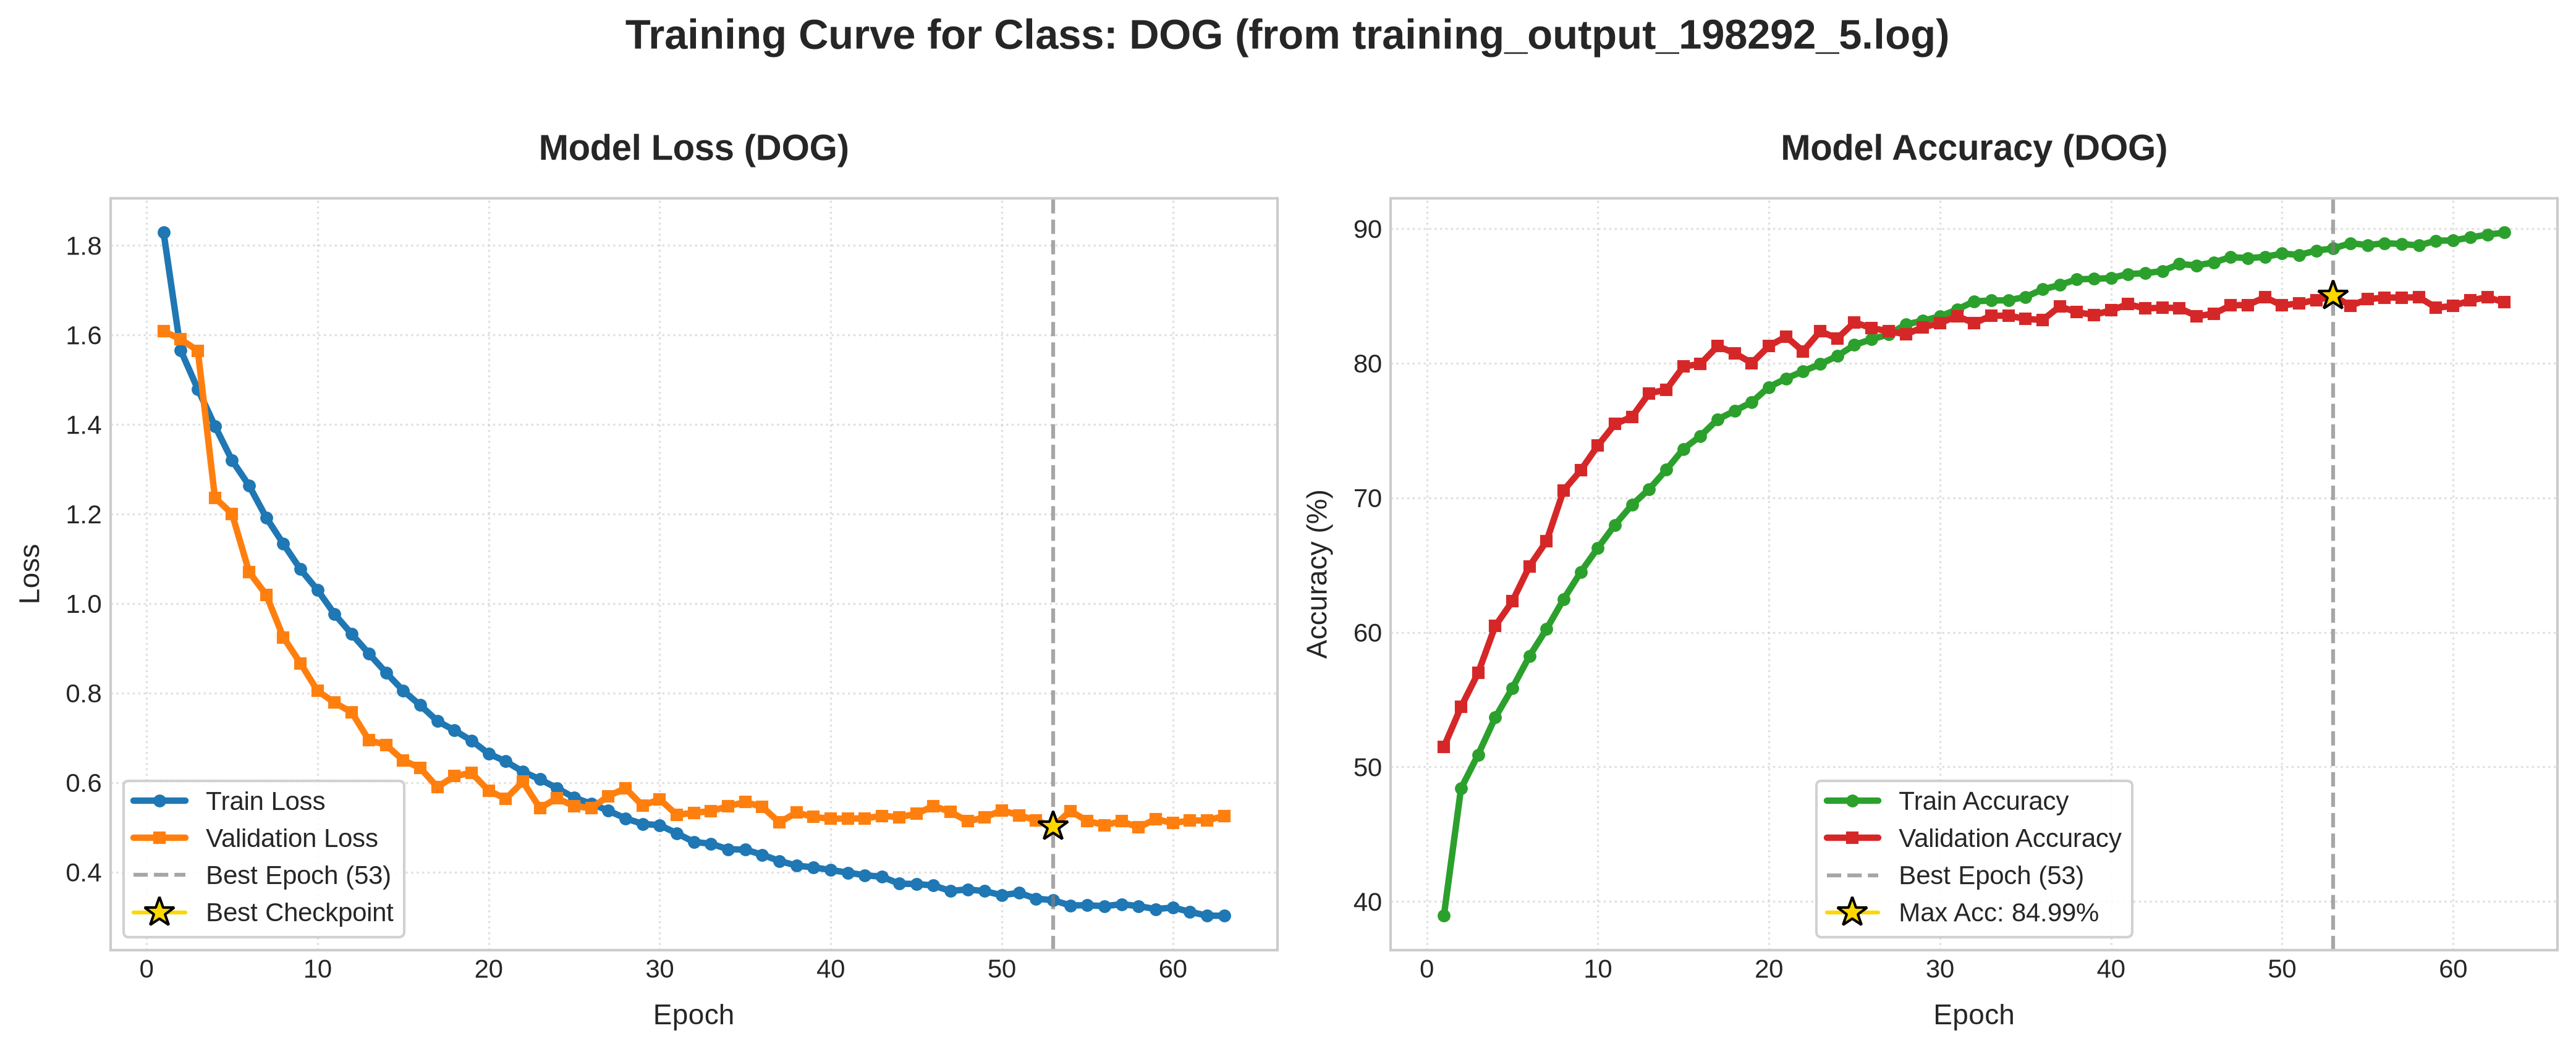
\includegraphics[width=\textwidth]{../Epoch/loss_Graphs/training_output_198292_5_dog.png}
        \caption{Task 5: Dog CropMix ($\text{LR}=1\times 10^{-5}$, 100 Ep., $84.99\%$)}
    \end{subfigure}
    \hfill
    \begin{subfigure}[b]{0.48\textwidth}
        \centering
        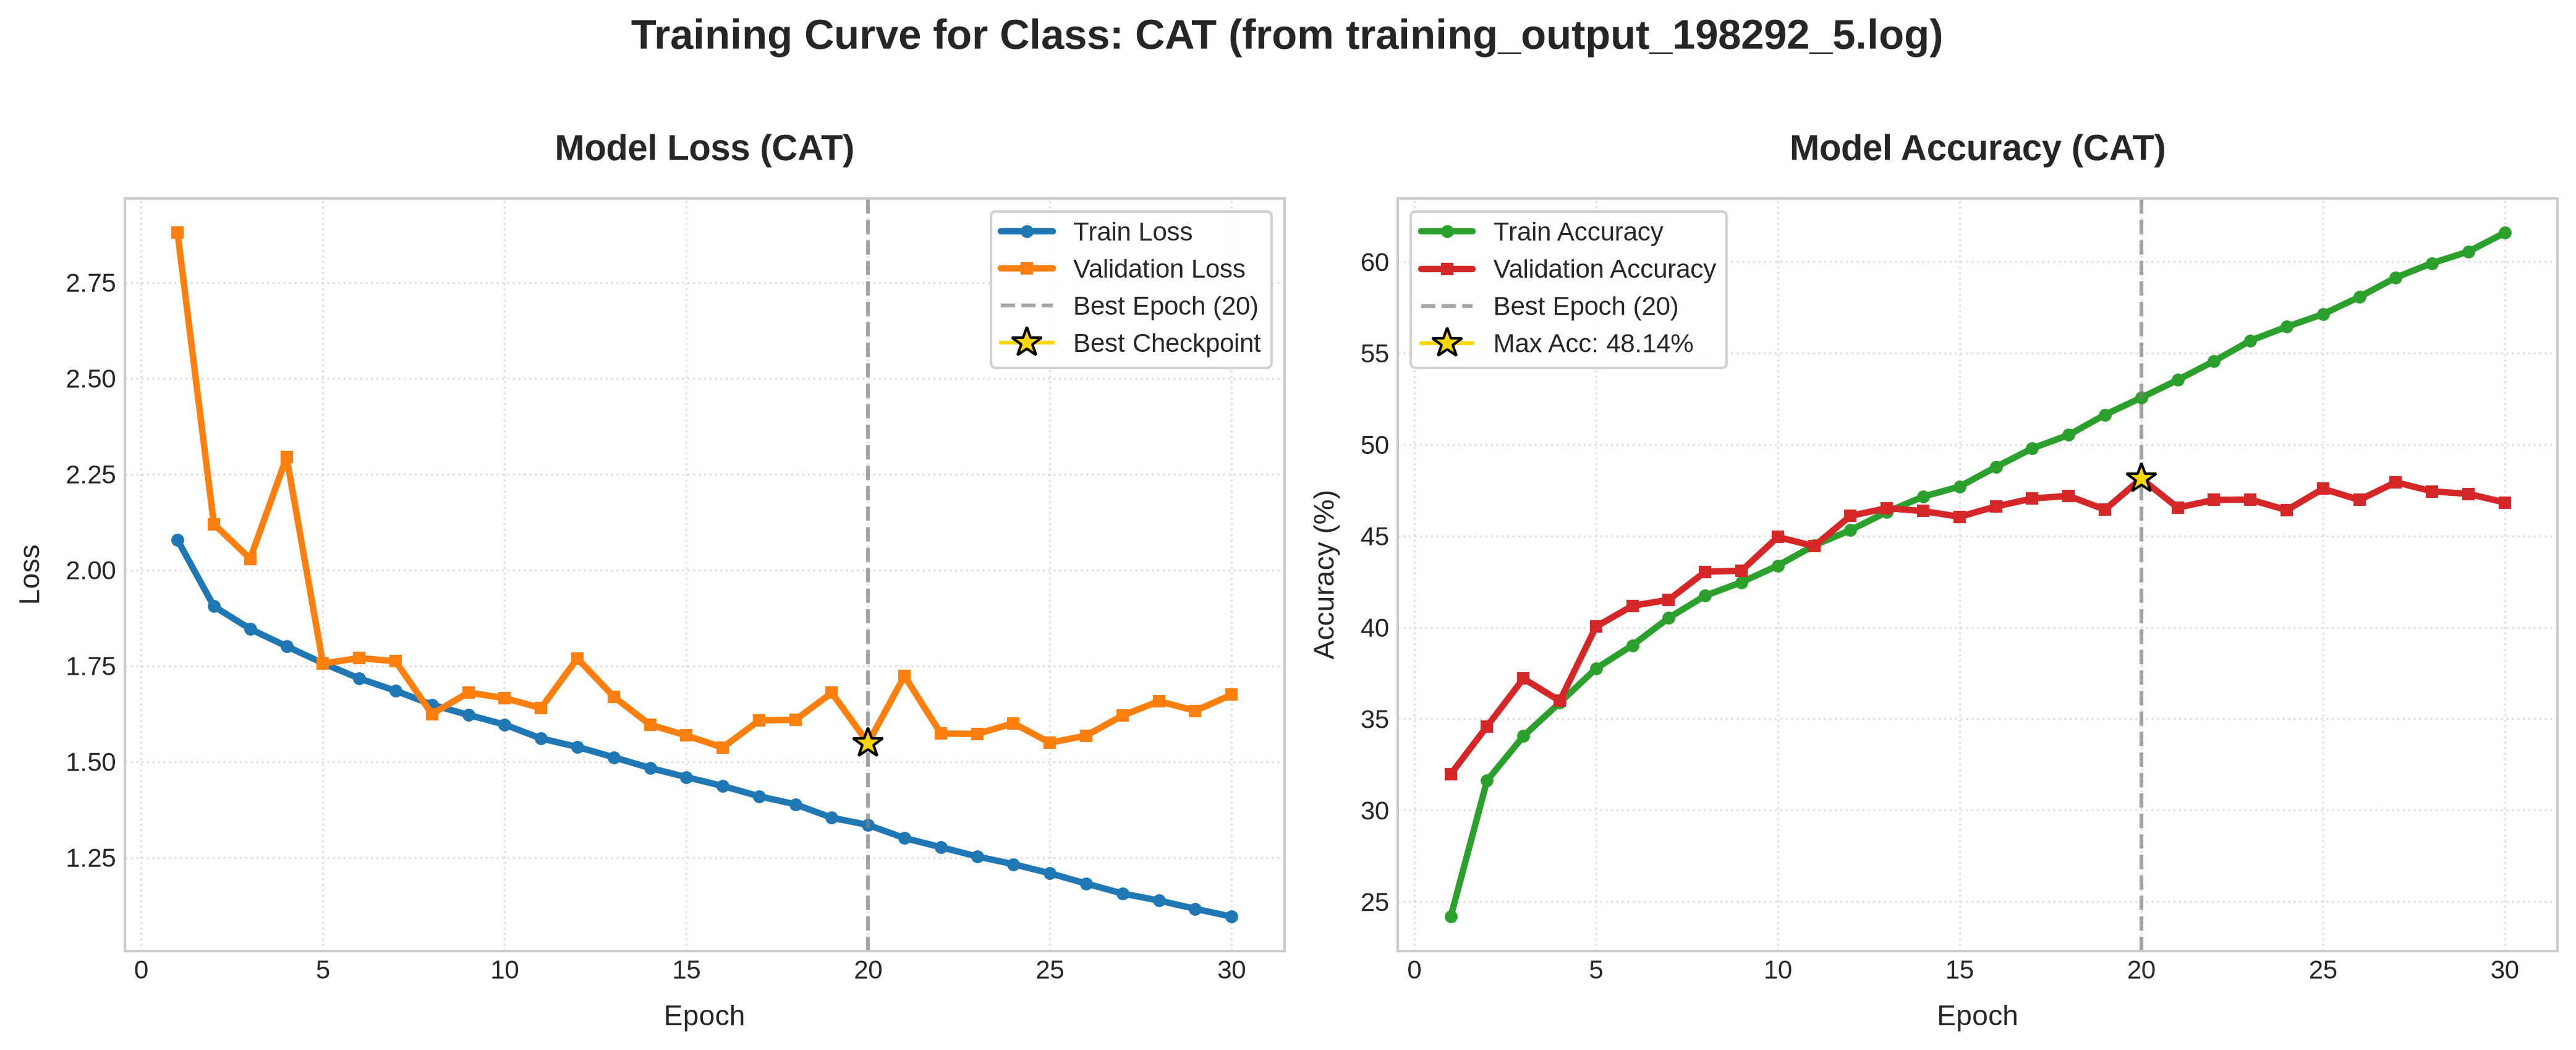
\includegraphics[width=\textwidth]{../Epoch/loss_Graphs/training_output_198292_5_cat.png}
        \caption{Task 5: Cat CropMix ($\text{LR}=1\times 10^{-5}$, 100 Ep.)}
    \end{subfigure}

    \vspace{0.3cm}

    % Task 6: All Augmentations Combined
    \begin{subfigure}[b]{0.48\textwidth}
        \centering
        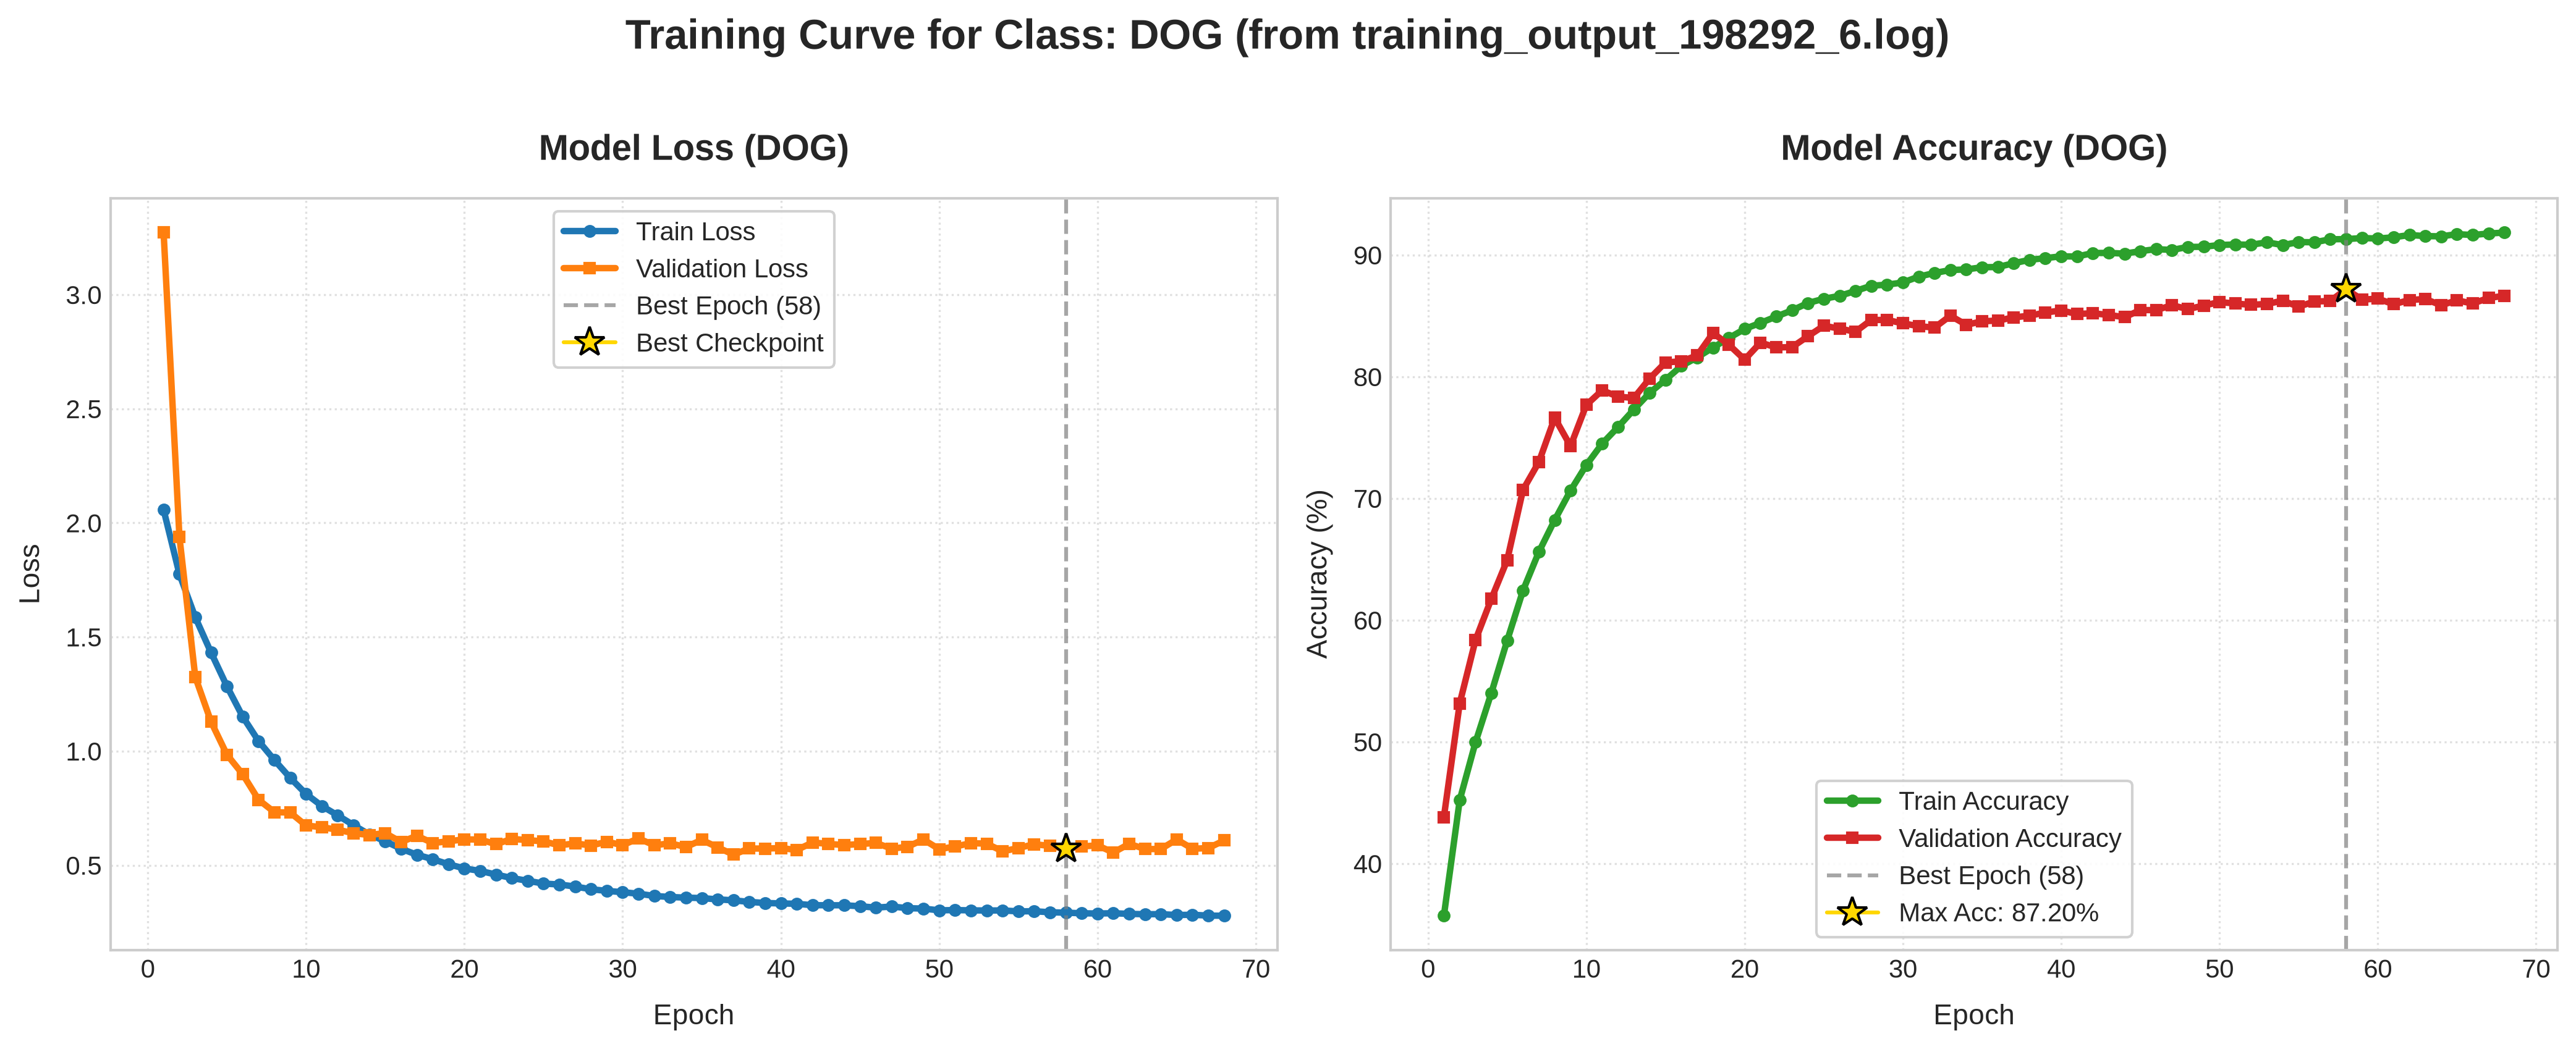
\includegraphics[width=\textwidth]{../Epoch/loss_Graphs/training_output_198292_6_dog.png}
        \caption{Task 6: Dog All Augs ($\text{LR}=1\times 10^{-5}$, 100 Ep.)}
    \end{subfigure}
    \hfill
    \begin{subfigure}[b]{0.48\textwidth}
        \centering
        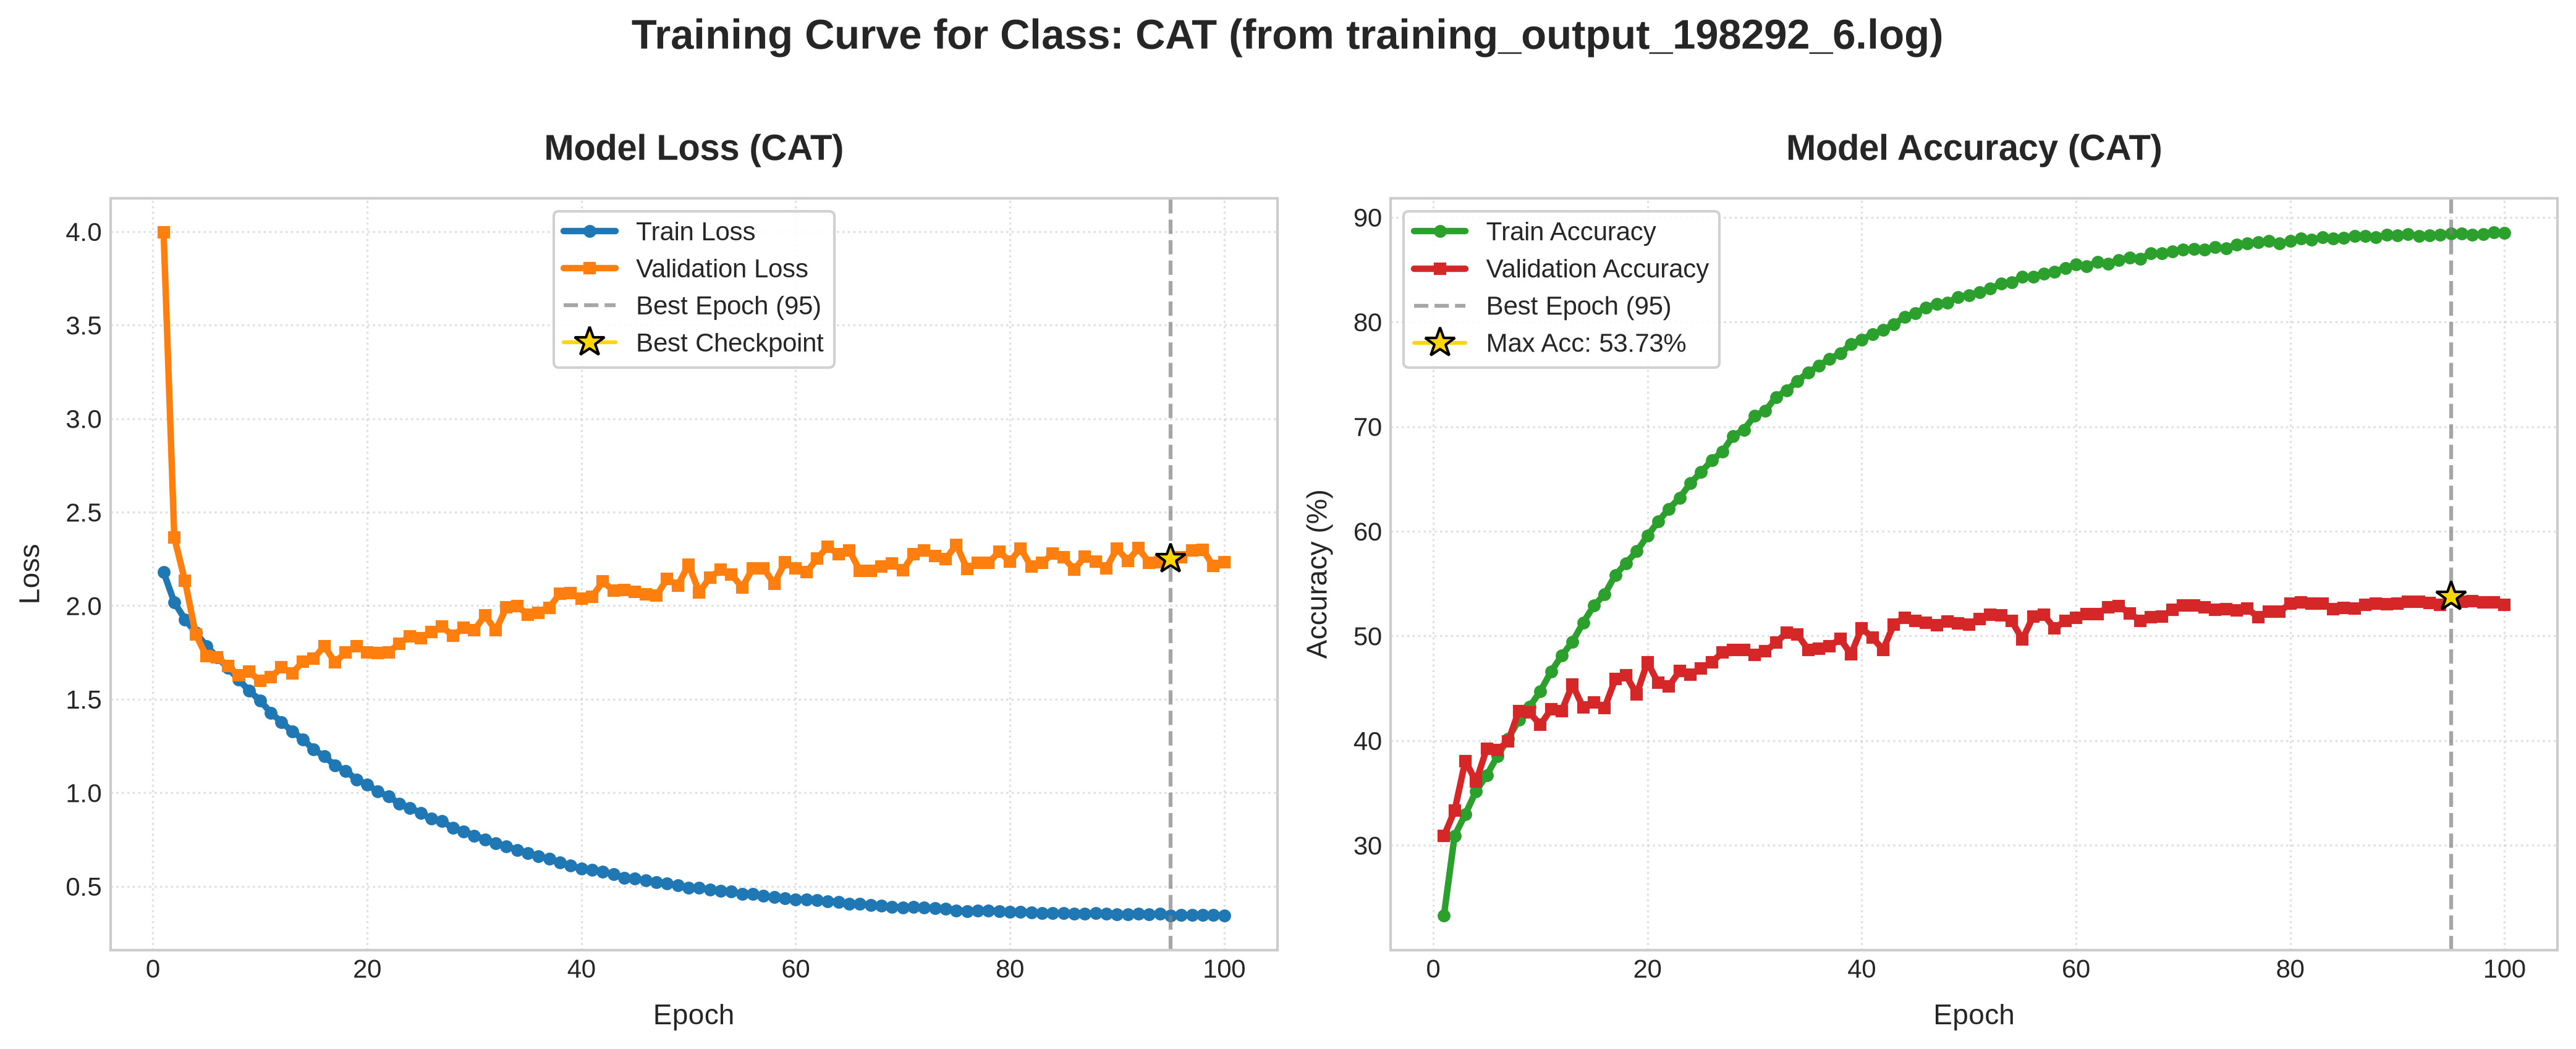
\includegraphics[width=\textwidth]{../Epoch/loss_Graphs/training_output_198292_6_cat.png}
        \caption{Task 6: Cat All Augs ($\text{LR}=1\times 10^{-5}$, 100 Ep., $53.73\%$)}
    \end{subfigure}

    \vspace{0.3cm}

    % Task 7: Long Run Baseline
    \begin{subfigure}[b]{0.48\textwidth}
        \centering
        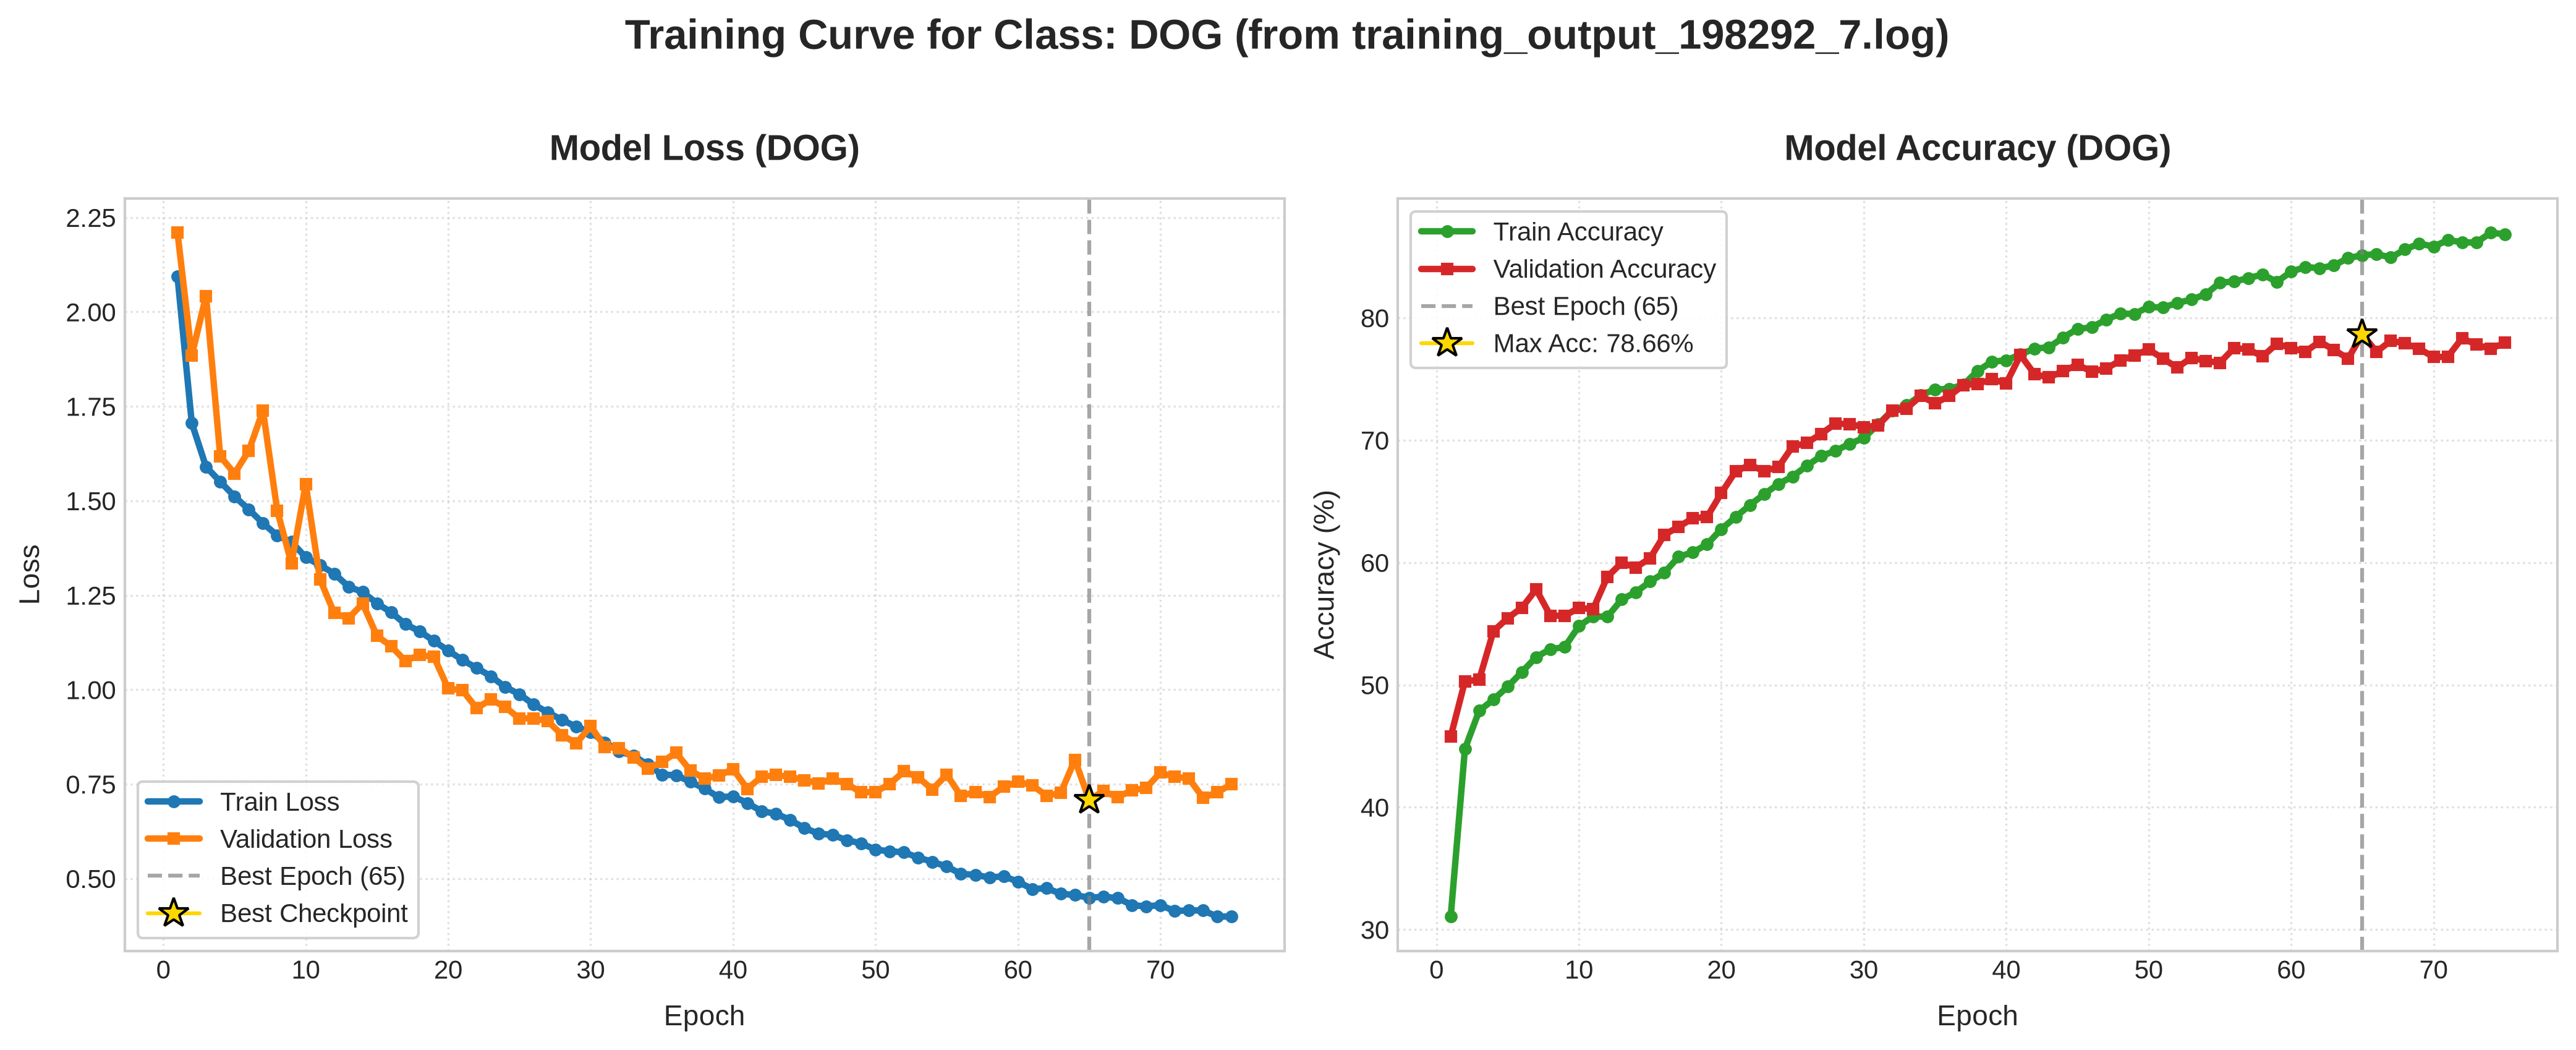
\includegraphics[width=\textwidth]{../Epoch/loss_Graphs/training_output_198292_7_dog.png}
        \caption{Task 7: Dog Extended Baseline ($\text{LR}=5\times 10^{-6}$, 1000 Ep., $78.66\%$)}
    \end{subfigure}
    \hfill
    \begin{subfigure}[b]{0.48\textwidth}
        \centering
        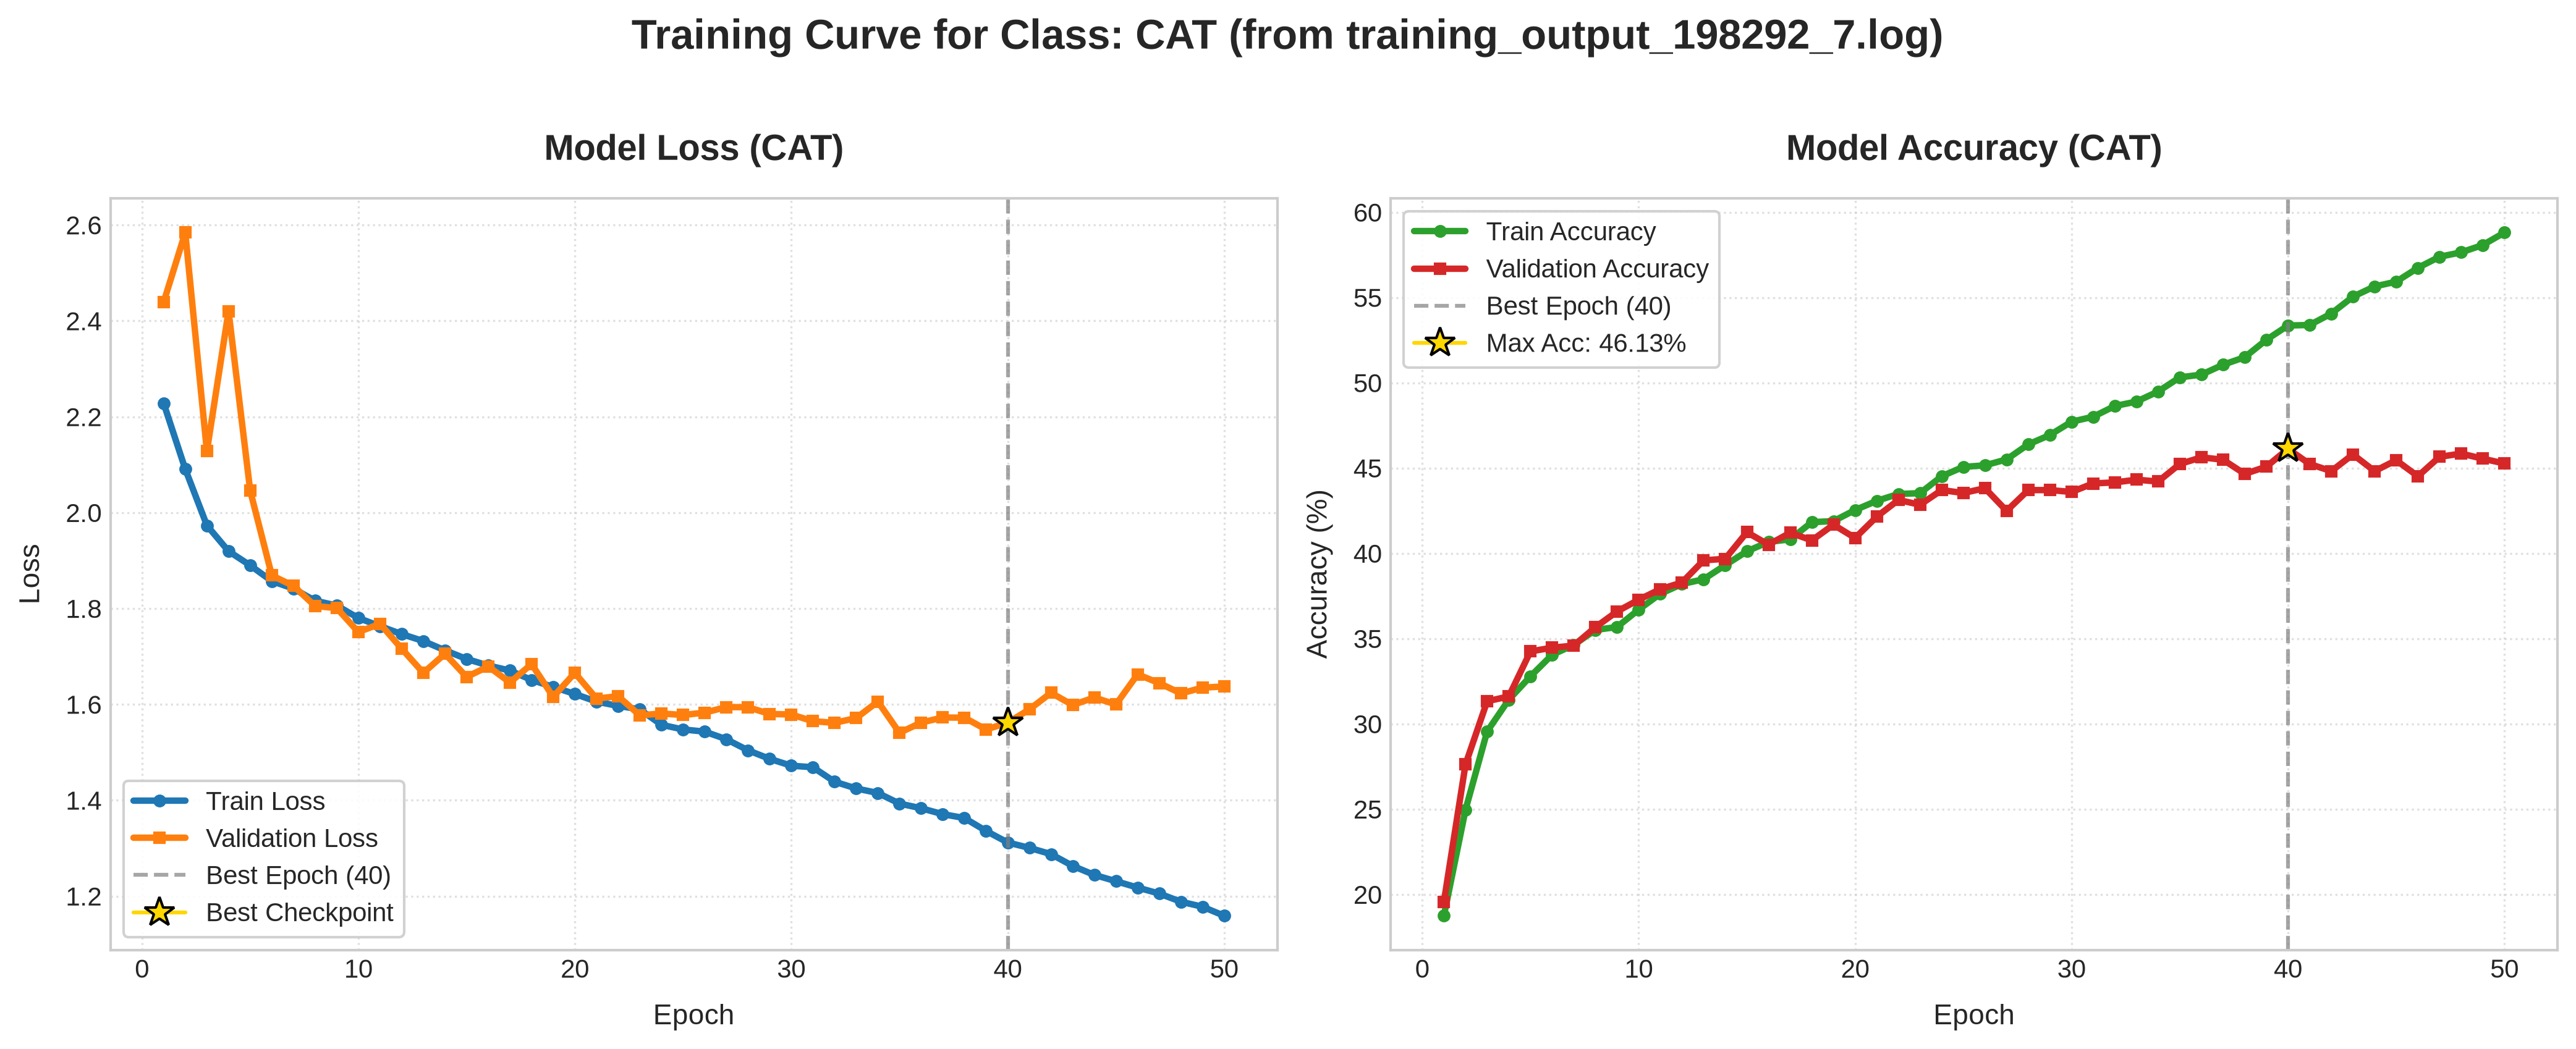
\includegraphics[width=\textwidth]{../Epoch/loss_Graphs/training_output_198292_7_cat.png}
        \caption{Task 7: Cat Extended Baseline ($\text{LR}=5\times 10^{-6}$, 1000 Ep., $46.13\%$)}
    \end{subfigure}
    
    \caption{Comprehensive comparison of training loss and accuracy dynamics across all Cat and Dog classification runs (Tasks 1--7) under various augmentation strategies and learning rates (all models trained from uninitialized weights).}
    \label{fig:appendix_training_curves}
\end{figure*}